
%% Vorlage fuer Studien- und Bachelorarbeiten an der HS Ravensburg-Weingarten
%% Benoetigt wird KOMA-Skript ab Version 2.8j vom 30.07.2001
%% Vor der Veraenderung irgendwelcher Einstellungen wird dringend empfohlen
%% die Anleitung zum KOMA-Skript (scrguide) zu konsultieren !!
%%
%% Bilder bitte nicht mit Endung einbinden, so ist die Erzeugung von
%% DVI, PS und PDF problemlos m�glich!
%% J. Moehler, 2008-12-10 
%%Kommentar


%% Dokumentendefinition
\documentclass[
   12pt,                % Schriftgroesse 12pt
   a4paper,             % Layout fuer Din A4
   german,              % deutsche Sprache, global   
%  twoside,             % Layout fuer beidseitigen Druck
	 oneside,						  % Layout für einseitigen Druck
   headinclude,         % Kopfzeile wird Seiten-Layouts mit beruecksichtigt
   headsepline,         % horizontale Linie unter Kolumnentitel
   plainheadsepline,    % horizontale Linie auch beim plain-Style
   BCOR12mm,            % Korrektur fuer die Bindung
   DIV18,               % DIV-Wert fuer die Erstellung des Satzspiegels, siehe scrguide
   halfparskip,         % Absatzabstand statt Absatzeinzug
   openany,             % Kapitel können auf geraden und ungeraden Seiten beginnen
   bibtotoc,            % Literaturverz. wird ins Inhaltsverzeichnis eingetragen
   pointlessnumbers,    % Kapitelnummern immer ohne Punkt
   tablecaptionabove,   % korrekte Abstaende bei TabellenUEBERschriften
   fleqn,               % fleqn: Glgen links (statt mittig)
%   draft               % Keine Bilder in der Anzeige, overfull hboxes werden angezeigt !Auskommentieren für Test-Compile!
]{scrbook}[2001/07/30]  % scrbook-Version mind. 2.8j von 2001/07/30

%% Pakete für nützliche Dinge
\usepackage{color} 							 % Schriftfarben verwenden
\usepackage{ngerman}             % neue deutsche Rechtschreibung
%\usepackage[ngerman]{translator} % Übersetzung 
%\usepackage[ansinew]{inputenc}   % Input-Encodung: ansinew fuer Windows
\usepackage[utf8]{inputenc}   % Input-Encodung: latin1 fuer Unix
\usepackage[T1]{fontenc}         % T1-kodierte Schriften, korrekte Trennmuster fuer Worte mit Umlauten
\usepackage{ae}                  % Für PDF-Erstellung
\usepackage[hang]{caption2}      % mehrzeilige Captions ausrichten
\usepackage{rotate}
\usepackage[centertags]{amsmath} % AMS-Mathematik, centertags zentriert Nummer bei split
\usepackage{longtable}
\usepackage{latexsym}            % verschiedene Symbole
\usepackage{textcomp}            % verschiedene Symbole
 \usepackage{microtype}          % bessere Optik     
\usepackage{graphicx}            % zum Einbinden von Grafiken
\usepackage{float}    
\usepackage{listings}           % u.a. genaue Plazierung von Gleitobjekten mit H
% \usepackage{pstricks}          % PostScript Macros
% \usepackage{lscape}            % Seite im Querformat bei Erhalt der Kopfzeile
% \usepackage{verbatim}          % Quellcode einbinden (\verbatiminput)
% \usepackage{multicol}          % Mehrspaltiger Text 
\usepackage{placeins}
\usepackage{pbox}
%%% Literatur und sonstige Referenzen
\usepackage{cite}              % Sortierte und zusammengefasste Zitatnummern 
\usepackage{url}							 % URL in Literatur wird unterst�tzt
\usepackage{varioref}          % Verbesserte Referenzen
\usepackage{hyperref}          % Verlinkte Verzeichnisse
\hypersetup{% 					%delet red boxes from hyperlink
	pdfborder = {0 0 0}
}

% \usepackage[numbers, sort]{natbib} % DIN Literaturverzeichnis; nicht zusammen mit cite verwenden!

%% Index
\usepackage{makeidx}						 % Index verwenden
\makeindex											 % index erstellen

%% Zeilenabstand
\usepackage{setspace}            % Zeilenabstand einstellbar
\onehalfspacing                  % eineinhalbzeilig einstellen

%% Kopf- und Fusszeilen
\usepackage{scrpage2}                             % Kopf und Fusszeilen-Layout 
\renewcommand{\headfont}{\normalfont\sffamily}    % Kolumnentitel serifenlos
\renewcommand{\pnumfont}{\normalfont\sffamily}    % Seitennummern serifenlos
\pagestyle{scrheadings}
\ihead[]{\headmark}               % Kolumnentitel immer oben innen
\chead[]{}                        % oben Mitte
\ohead[\pagemark]{\pagemark}      % Seitennummern immer oben aussen
\ofoot[]{}                        % Fusszeile aussen
\cfoot[]{}                        % Fusszeile Mitte
\ifoot[]{}                        % Fusszeile innen

%% Fussnotenzähler
\usepackage{chngcntr}              % Paket um Counter zu steuern
\counterwithout{footnote}{chapter} % Fussnoten nicht pro Chapter, sondern Global
\usepackage{threeparttable}        % Tabelle mit Fussnoten

%% Namen von Verzeichnissen definieren
\renewcommand{\bibname}{Literatur}               % Literaturverzeichnis wird zu Literatur
\renewcommand{\figurename}{Bild}                 % Abbildung wird zu Bild
\renewcommand{\listfigurename}{Bildverzeichnis}
\renewcommand{\indexname}{Stichwortverzeichnis}

%% Schrift mit Serifen auch fuer Ueberschriften benutzen
%\renewcommand*{\sectfont}{\bfseries}
%\renewcommand*{\descfont}{\bfseries}

\typearea[current]{current}        % Neuberechnung des Satzspiegels mit alten Werten nach Änderung von Zeilenabstand,etc

% -- Glossar --
\usepackage[toc, acronym]{glossaries} % Glossareinträge, muss nach hyperref (insofern dies verwendet wird) geladen werden
% (aufgrund der Seitenzahlverlinkung im Glossarverzeichnis), (benötigt die Packete
% "xkeyval" und "supertabular", welche dann automatisch eingebunden werden)
%\newglossary[slg]{symbolslist}{syi}{syg}{Symbolverzeichnis} %Ein eigenes Symbolverzeichnis erstellen
\renewcommand*{\glspostdescription}{} %Den Punkt am Ende jeder Beschreibung deaktivieren
\makeglossaries % erstellt ein Glossar (Verzeichnis für Begriffserklärungen,
% z.B.: Abkürzungen)
% Glossareinträge (MUSS für JEDEN Glossareintrag überarbeitet werden):
%% Symbole:
%%\newglossaryentry{symb:Name}{name=Symbolname, description={Beschreibung}, sort=alphabetisches Wort für die Einreihung, type=symbolslist}
\newglossaryentry{symb:Pi}{
name=$\pi$,
description={Die Kreiszahl.},
sort=symbolpi, type=symbolslist
}
%%Abkürzungen:
%%\newacronym{Referenz}{Abkürzung}{Beschreibung}
\newacronym{BSP}{BSP}{Beispiel}


%%Eine Abkürzung mit Glossareintrag:
%%\newacronym{Referenz}{Abkürzung}{Beschreibung\protect\glsadd{glos:Referenz}}
\newacronym{AD}{AD}{Active Directory\protect\glsadd{glos:AD}}

%%Glossareintrag:
%%\newglossaryentry{glos:Referenz}{name=Name, description={Beschreibung}}
\newglossaryentry{glos:AD}{
name=Active Directory,
description={Active Directory ist in einem Windows Server 2000, Windows
Server 2003, oder Windows Server 2008-Netzwerk der Verzeichnisdienst, 
der die zentrale Organisation und Verwaltung aller Netzwerkressourcen erlaubt. Es
ermöglicht den Benutzern über eine einzige zentrale Anmeldung den
Zugriff auf alle Ressourcen und den Administratoren die zentral
organisierte Verwaltung, transparent von der Netzwerktopologie und
den eingesetzten Netzwerkprotokollen. Das dafür benötigte
Betriebssystem ist entweder Windows Server 2000, 
Windows Server 2003, oder Windows Server 2008, welches auf dem zentralen
Domänencontroller installiert wird. Dieser hält alle Daten des
Active Directory vor, wie z.B. Benutzernamen und
Kennwörter.}
}

\newglossaryentry{glos:Glossareintrag}{name=Glossareintrag, description={Erweiterte Informationen zum
einem Wort oder einer Abkürzung, ähnlich einem Eintrag im Duden.}}




%%% Local Variables: 
%%% mode: latex
%%% TeX-master: "Bachelorarbeit"
%%% End: 
\usepackage[left = 2.54cm, right = 2.54cm]{geometry}
%%% PDF-Erzeugung: pdflatex statt latex aufrufen!
%% BEI WINDOWS UND TEXNICCENTER AUSKOMMENTIERT LASSEN !!! 
%\pdfoutput=1                  % PDF-Ausgabe
%\usepackage[pdftex, a4paper,  % muss letztes Package sein!
%     pdftitle={Titel der Arbeit},%
%     pdfauthor={Name Autor},%
%     pdfsubject={Studien- bzw. Diplomarbeit},%
%     pdfkeywords={Stichwort zur Arbeit},%
%    ]{hyperref} % 



%\graphicspath{{figs/}{bilder/}}    % Falls texinput nicht gesetzt -> Bildverzeichnisse

%\includeonly{}

\definecolor{mygreen}{rgb}{0,0.6,0}
\definecolor{mygray}{rgb}{0.5,0.5,0.5}
\definecolor{mymauve}{rgb}{0.58,0,0.82}

\lstset{ 
	backgroundcolor=\color{white},   % choose the background color; you must add \usepackage{color} or \usepackage{xcolor}; should come as last argument
	basicstyle=\footnotesize\ttfamily,        % the size of the fonts that are used for the code
	breakatwhitespace=false,         % sets if automatic breaks should only happen at whitespace
	breaklines=true,                 % sets automatic line breaking
	captionpos=b,                    % sets the caption-position to bottom
	commentstyle=\color{mygreen},    % comment style
	deletekeywords={...},            % if you want to delete keywords from the given language
	escapeinside={\%*}{*)},          % if you want to add LaTeX within your code
	extendedchars=true,              % lets you use non-ASCII characters; for 8-bits encodings only, does not work with UTF-8
	%firstnumber=1000,                % start line enumeration with line 1000
	%frame=single,	                   % adds a frame around the code
	keepspaces=true,                 % keeps spaces in text, useful for keeping indentation of code (possibly needs columns=flexible)
	keywordstyle=\color{blue},       % keyword style
	language=Python,                 % the language of the code
	morekeywords={self,*},            % if you want to add more keywords to the set
	%numbers=left,                    % where to put the line-numbers; possible values are (none, left, right)
	%numbersep=5pt,                   % how far the line-numbers are from the code
	%numberstyle=\tiny\color{mygray}, % the style that is used for the line-numbers
	%rulecolor=\color{black},         % if not set, the frame-color may be changed on line-breaks within not-black text (e.g. comments (green here))
	showspaces=false,                % show spaces everywhere adding particular underscores; it overrides 'showstringspaces'
	showstringspaces=false,          % underline spaces within strings only
	showtabs=false,                  % show tabs within strings adding particular underscores
	%stepnumber=2,                    % the step between two line-numbers. If it's 1, each line will be numbered
	stringstyle=\color{mymauve},     % string literal style
	tabsize=2,	                   % sets default tabsize to 2 spaces
	title=\lstname                   % show the filename of files included with \lstinputlisting; also try caption instead of title
}
\setcounter{secnumdepth}{4}
\usepackage{titlesec}
\titleformat{\paragraph}
{\normalfont\normalsize\bfseries}{\theparagraph}{1em}{}
\titlespacing*{\paragraph}
{0pt}{3.25ex plus 1ex minus .2ex}{1.5ex plus .2ex}
%%%%%%%%%%%%%%%%%%%%%%%%%%%%%%%%%%%%%%%%%%%%%%%%%%%%%%%%%%%%%%%
\begin{document}

\pagenumbering{Roman}           % Nummerierung Römisch Start bei I

%% Deckblatt fuer Studien- und Diplomarbeiten am der
%% Hochschule Weingarten

\thispagestyle{empty}
%~
{
\normalsize\fontfamily{phv} \fontsize{12pt}{10}\selectfont 
\vspace{-1cm}
\begin{minipage}[b]{9.4cm}
{\fontsize{13pt}{13} \selectfont%
Hochschule\\[1ex]
Ravensburg-Weingarten}\\[1ex]
\end{minipage}
}
\begin{minipage}[b]{10cm}
\includegraphics*[height=2.7cm]{bilder/HSLogoWGd}
\end{minipage}


\vspace{10mm}
 
\hrule 
\vspace{1cm}
{
\fontseries{b} \fontsize{20pt}{20}  \selectfont%
\begin{center}
\textcolor{red}{Titel der Arbeit} % Titel der Arbeit
\end{center}
}

\begin{center}
\large \textbf{Dokumentation zu Seminar} % Hier Praxisarbeit, Studienarbeit, Bachelorarbeit, Dokumentation zu Seminar, etc. eintragen
\end{center}

\begin{center}
\textbf{Multimedia Technik SS09} % Hier den Zusatz wie Fach oder Semester eintragen
\end{center}

\vspace{5mm}

\begin{center}
im Studiengang \textcolor{red}{Angewandte Informatik} % Hier den Studiengang eintragen
\end{center}

\begin{center}
an der Hochschule Ravensburg - Weingarten 
\end{center}
\begin{center}

\end{center}
\vspace{5mm}
\begin{center}
von
\end{center}




\begin{center}
{\fontsize{12pt}{12} \selectfont%
\begin{tabular}{ll}
Autor Name & \textcolor{red}{Matr.-Nr.: xxxxx}\\[0.5ex] % Hier den Autor und die Matrikelnummer statt xxxxx eintragen
%Autor 2 & \textcolor{red}{Matr.-Nr.: xxxxx}\\[0.5ex] % Für weitere Autoren Zeilen auskommentieren bzw. kopieren und ausfüllen
%Autor 3 & \textcolor{red}{Matr.-Nr.: xxxxx}\\[0.5ex]
Abgabedatum :& \today   % Das Abgabedatum wird gleichgesetzt mit dem Datum der letzten Compilierung. Statt \today kann auch Datum von Hand geschrieben werden
\end{tabular}
}
\end{center}
                               

\vspace{1cm}

\vspace{1cm}
\hrule


%%% Local Variables: 
%%% mode: latex
%%% TeX-master: "Bachelorarbeit"
%%% End: 

                % Deckblatt Nummerierung unterdrückt (In Deckblatt festgelegt)
%%\cleardoubleemptypage         % Die Eidesstattliche Erklaerung auf einer rechten Seite beginnen
%% Eidestattliche Erklärung %%
%% Die Erklärung sollte nach dem Deckblatt fest abgeheftet werden
\addchap*{Erklärung} %* nicht entfernen, sonst erhält Erklärung eine Nummer und erscheint im Inhaltsverzeichnis

\thispagestyle{empty} %Keine Seitenzahl, keine Kopf- und Fusszeile

Hiermit erkläre ich, dass ich die vorliegende Arbeit mit dem Titel   % ein Autor
% Hiermit erkl"aren wir, dass wir die vorliegende Arbeit mit dem Titel \newline % mehrere Autoren
\begin{center}
\textbf{Entwicklung einer Anwendung zur automatisierten Beschaffung von personenbezogenen Daten im Internet und deren Integration in Phishing-Mails}
\end{center}
selbstständig angefertigt, nicht anderweitig zu Prüfungszwecken vorgelegt, keine anderen als die angegebenen Hilfsmittel benutzt und wörtliche sowie sinngemäße Zitate als solche gekennzeichnet habe.\newline  % ein Autor

\begin{flushleft}
Weingarten, 29. April 2019 % Ort eintragen, /today kann durch Datum 2009-10-21 oder 21.10.2009 ersetzt werden
\end{flushleft}

%%% Unterschriftenblock für einen Autor
\begin{tabular}{l}   
Autor Name        \\% Hier Autor eintragen
 \\
------------------------------------ \\
\end{tabular}

%%% Unterschriftenblock für mehrere Autoren
%\begin{tabular}{lll}
%Autor 1       &Autor 2      &Autor 3 \\% Hier eintragen
% & & \\
%------------------------------------ & ------------------------------------ & ------------------------------------ \\
%\end{tabular}

%Hier unterschreiben


%%% Local Variables: 
%%% mode: latex
%%% TeX-master: "Bachelorarbeit"
%%% End: 
                 % Eidesstattliche Erklaerung Nummerierung unterdrückt
%%\cleardoubleemptypage         % Das Inhaltsverzeichnis auf einer rechten Seite beginnen

\pagenumbering{Roman}           % Nummerierung Römisch start bei I 

\begin{spacing}{1.0}            % Verzeichnisse werden mit einzeiligem Abstand gesetzt
 \tableofcontents               % Inhaltsverzeichnis
\end{spacing}
%%% Vorbemerkungen %%%  Nummerierung unterdrückt durch *
\addchap{Kurzfassung}
\label{cha:kurzfassung} 
Es wird gezeigt, wie eine automatisierte Suche nach personenbezogenen Daten im Internet aussehen kann und wie diese Daten für einen Phishing-Mail-Angriff verwendet werden können. 

Wird erweitert!

%%% Local Variables: 
%%% mode: latex
%%% TeX-master: "Bachelorarbeit"
%%% End: 


             % Kurzfassung der Arbeit
%\addchap{Abstract}
\label{cha:abtract} 







%%% Local Variables: 
%%% mode: latex
%%% TeX-master: "Bachelorarbeit"
%%% End: 
             % Abstract der Arbeit (englische Kurzfassung der Arbeit)
\addchap{Danksagung}
\label{cha:danksagung}



%%% Local Variables: 
%%% mode: latex
%%% TeX-master: "Bachelorarbeit"
%%% End: 								  % Danksagung (optional)
%\addchap{Vorwort}
\label{cha:vorwort}



%%% Local Variables: 
%%% mode: latex
%%% TeX-master: "Bachelorarbeit"
%%% End: 							    % Vorwort (optional)

%%% Hauptteil %%%       Nummerierung beginnend bei 1
%%\cleardoubleplainpage         % Das erste Kapitel des Hauptteils auf einer rechten Seite beginnen
\mainmatter                     % den Hauptteil beginnen
\chapter{Einleitung}
\label{cha:einleitung}

%%% Local Variables: 
%%% mode: latex
%%% TeX-master: "Bachelorarbeit"
%%% End: 

\section{Motivation}
\label {sec:Motivation}
In der heutigen Zeit wird das Thema Informationssicherheit immer wichtiger. Systeme werden immer komplexer und Firewalls immer besser.
Doch laut dem Bundeskriminalamt hat sich die Zahl der Cyberkriminalität mit einem klaren Trend nach oben entwickelt. \cite{Cyberkriminalitaet}\\
Eine häufig verwendetet Technik von Cyberkriminalität ist das E-Mail-Phishing. Hier wird der Mensch als Schwachstelle des Systems genutzt. In den neusten Fällen von Phishing-Attacken zeigt die Verbraucherzentrale Nordrhein-Westfalen, dass diese meist direkt an eine Person adressiert sind. Beispielsweise wird man in den gefälschten DSGVO-E-Mails, im Namen der Sparkasse, persönlich mit Namen angesprochen. \cite{VerbraucherzentraleNW} \\
Im Rahmen dieser Abschlussarbeit wird gezeigt, mit welchem Aufwand solche Angriffe verbunden sind und wie die Suche nach privaten Informationen im Internet aussieht.

\section{Problem}
Leser Problem komplett erklären, weiterführende Motivation

Persönliche Informationen werden im Internet immer leichter zugänglich gemacht. !!!ZITAT!!!\\
Es gibt viele Webseiten die persönliche Information von Menschen bereitstellt. Eine davon ist auch www.fupa.net. Hier können persönliche Informationen ohne Anmeldung ausgelesen werden. Diese Art von Webseite ist eine perfekte Informationsquelle für Angreifer.\\
Im Bereich von Social Engineering Angriffen wird diese Information oft genutzt um ein Opfer zu manipulieren.
Das hier beschriebene Problem zeigt dass der Zugang für persönliche Information durch das Internet für viele Menschen einfacher gemacht wird. Es soll gezeigt werden wie einfach es ist, personenbezogene Daten aus dem Internet herauszulesen, analysieren und für einen Phishing-Angriffe zu verwenden.
!!!!ZITATE HINZUFÜGEN!!! statista z.B.

\section{Eigene Leistung}
\label {sec:Leistung} 
In dieser Arbeit wird ein Phishing-Mailgenerator erstellt. Dieser liest automatisiert Informationen von der Webseite www.fupa.net heraus und erstellt potentiellen Opferprofile. Zusätzlich wird mit dieser Information und einem Web-Crawler das Internet nach weiteren Informationen durchstöbert. Mit dem Vornamen, Nachnamen und dem Geburtsjahr werden die E-Mail-Adressen generiert. Die gefundenen Informationen werde automatisch in eine personalisierte Phishing-E-Mail eingebaut. Für einen höheren Erfolg werden E-Mail-Muster erstellt.

\section{Aufbau der Arbeit}
\label {sec:Aufbau} 
Meine Arbeit gliedert sich in zwei Teile. Einem theoretischen und einem praktischen Teil. Der Theorie-Teil beginnt im zweiten Kapitel und beschreibt die Grundbegriffe im Bereich Social Engineering, Webtools, E-Mails und Programmiersprachen. Im nächsten Kapitel befindet sich die Anforderungsanalyse. Hier werden die Anforderungen an die Arbeit festgelegt. Darauf folgen die Lösungsvorschläge im Kapitel vier und die ausgewählte Lösung anhand den Anforderungen im Kapitel 5. Im Anschluss wird bei der Umsetzung auf den Praktischen Teil eingegangen.Am Ende befindet sich das Fazit, der Ausblick und der Anhang.






               % Einleitung
%Kapitel des Hauptteils

\chapter {Grundlagen}  %Name des Kapitels
\label{cha:grundlagen} %Label des Kapitels

\section{Personenbezogene Daten}
%TODO möglicherweise unterschied von Information und Daten erklären
Laut dem DSGVO sind \textit{personenbezogene Daten} 

\textit{"'alle Informationen, die sich auf eine identifizierte oder identifizierbare natürliche Person (im Folgenden „betroffene Person“) beziehen; als identifizierbar wird eine natürliche Person angesehen, die direkt oder indirekt, insbesondere mittels Zuordnung zu einer Kennung wie einem Namen, zu einer Kennnummer, zu Standortdaten, zu einer Online-Kennung oder zu einem oder mehreren besonderen Merkmalen identifiziert werden kann, die Ausdruck der physischen, physiologischen, genetischen, psychischen, wirtschaftlichen, kulturellen oder sozialen Identität dieser natürlichen Person sind;"'}\cite{personenbezogeneDaten}

\section{Social Engineering} %Unterkapitel
\label {sec:Social Engineering} %Label des Unterkapitels
	Die Definition von Social Engineering (SE) ist nicht eindeutig. Es gibt sehr verschiedene Ansichten von der Definition. Die Idee von Social Engineering ist, eine Ziel so zu manipulieren, damit das Ziel eine für den Angreifer bessere Entscheidung trifft. In dem Buch Social Engineering - The Art of Human Hacking, von Christopher Hadnagy, ist Social Engineering definiert als:
	
	\textit{"'social engineering is the act of manipulating a person to take an action that may or may not be in the "'target’s"' best interest"'}\cite{ArtOfHumanHacking}
	
	Wiederum lautet die Definition in dem Buch von Kevin D. Mitnick:
	
	\textit{"'Social Engineering uses influence and persuasion to deceive people by convincing them that the social engineer is someone he is not, or by manipulation. As a result, the social engineer is able to take advantage of people to obtain information with or without the use of technology"'}\cite{ArtOfDeception}
	
	SE wird Menschen von Geburt an beigebracht und begegnet einem beinahe jeden Tag. Schon ein Baby muss wissen wie es die Eltern manipulieren kann damit es Dinge wie Essen, Zuneigung, o.ä. bekommt. Darüber hinaus ist SE in vielen Berufen ein täglicher Bestandteil. Beispielsweise manipulieren Ärzte viele Patienten mit einer Placebo-Behandlung. Bei dieser Behandlung wird dem Patient ein wirkstoff-freies Medikament verschrieben. Ausschließlich durch die Manipulation des Patienten und den sogenannten Palzebo-Effekt können Erfolge erzielt werden.
	
	Im Bereich der Informationssicherheit, wird von Social Engineering gesprochen, wenn Angreifer durch die Manipulierung und Täuschung von Menschen vertrauliche Informationen oder Zugänge zu Systemen bekommen. Die bekanntesten Angriffsmethoden sind Phishing, Pretexting, Baiting und Quad Pro Quo. Bei dieser Arbeit wird hauptsächlich auf das Thema E-Mail-Phishing eingegangen.

	Der Aufbau eines SE-Angriffes ist definiert in mehrere Phasen. Das wohl bekannteste Modell für einen Social Engineering-Angriffszyklus ist in dem Buch von Kevin D. Mitnicks \cite{ArtOfDeception} definiert. Dieser Zyklus besteht aus den 4 Phasen \textit{Research, Developing rapport and trust, Exploiting trust} und \textit{Utilize information}.\\
	In der \textit{Research-Phase} geht es um die Informationsbeschaffung. Bei dieser Phase will der Angreifer möglichst viel Informationen über das Ziel herausfinden. Die \textit{Developing Rapport and Trust-Phase} beschreibt den Kontaktaufbau zum Ziel, da wenn das Opfer dem Angreifer vertraut, hat dieser ein leichteres Spiel in den kommenden Phasen. Das nun erzeugte Vertrauen wird in der \textit{Exploitung Trust-Phase} ausgenutzt. Hier will der Angreifer die eigentlich Information vom Opfer herausfinden. Dies geschieht einerseits durch bestimmtes Nachfragen oder Manipulation.
	\textit{Utilize Information} ist die letzte Phase. Dort wird die gewonnene Information genutzt um das eigentliche Ziel des Angreifers zu erreichen.\\
	Grundsätzlich werden bei einem Social Engineering Angriff menschliche Wünsche, Ängste und verbreitete Verhaltensmuster verwendet um ein Opfer zu manipulieren.\cite{LeitfadenSE}\\

		\subsection{Phishing}
		Das Wort Phishing wird von dem Wort "'fishing"' abgeleitet, da die Angreifer nach Informationen fischen. Das "'Ph"' kommt von "'sophisticated"' und meint damit, dass die Angreifer ausgeklügelte Techniken verwenden um an Informationen heranzukommen.\cite{PhishingExposed}\\
		Die wohl bekannteste Angriffsmethode von Phishing ist das E-Mail-Phishing. Bei diesem Verfahren, versendet ein Angreifer meist eine gefälschte E-Mail, um ein Opfer zu täuschen und dadurch sein Ziel zu erreichen. Die sogenannten Phishing-Mails enthalten meist eine Aufforderung einen Link zu öffnen und sehen täuschend echt aus. Zum Beispiel könnte der Angreifer ein Layout von Amazon verwenden und das Ziel auffordern, den Link zu öffnen wegen einem Authentifizierungsproblem. Nachdem Sie auf den Link geklickt haben müssen Sie sich anmelden. Hier könnten die Angreifer Ihre Anmeldedaten abgreifen, nachdem sie das Opfer eingeben hat. Sobald die Anmeldedaten eingegeben wurden, könnte eine Fehlermeldung erscheinen, die sagt: "'Hoppla, ein Fehler ist aufgetreten, melden Sie sich bitte neu an!"'. Anschließend wird die originale Seite geladen, das Opfer kann sich korrekt anmelden und der Angreifer hat ohne einen großen Aufwand die Anmeldedaten der Zielperson.\\
		Für diese Methode benötigt der Angreifer nicht nur Social Engineering  sondern auch technische Fähigkeiten.\cite{PhishingDarkWaters}
		
		\subsubsection{Spear-Phishing}
		Das Spear-Phishing ist eine erweiterte Methode des herkömmlichen E-Mail-Phishings. Hierbei wird anstatt das Versenden etlicher Phishing-Mails an unbekannte Opfer, eine gezielte Mail an eine ausgewählte Person versendet.\cite{SpearPhishingPaper}\\
		Bei dieser Form von E-Mail-Phishing spielt die Opferauswahl und die Informationsbeschaffung eine wichtig Rolle, da diese Information später für personalisierte E-Mails oder vorgetäuschte Identitäten verwendet werden können. Durch diese Art von Täuschung kann ein Opfer dazu bewegt werden auf einen Link zu klicken und dadurch eine Schadsoftware herunterzuladen.\cite{SpearPhishingPaper} \\
		Der Aufwand für die Informationsbeschaffung wird oft in Kauf genommen, da der Erfolg bei dieser Methode vielversprechender ist als beim herkömmlichen E-Mail-Phishing.\\
		91\% der Advanced Persistent Threat (APT) Angriffe auf Firmen beginnen mit einer Spear-Phishing-E-Mail. Die Schadsoftware wir meisten als Remote Access Trojans (RATs) in einem Zip-Datei überliefert.\cite{SpearPhishing}


\section{Informationsbeschaffung im Internet}
%TODO Entweder Web Crawling und Web Scraping oder Web Crawler und Web Scraper
	\subsection{Web Crawler}
		Web Crawler sind Computerprogramme, die mit Hilfe der Hypertextstruktur das Internet durchlaufen. Dabei können sie in einen \textbf{internen} und \textbf{externen Web Crawler} unterschieden werden. Der interne Web Crawler durchsucht ausschließliche interne Seiten einer Webseite und der externe Web Crawler durchsucht unbekannte Webseiten im ganzen Netz. \cite{sharma2012study}

		In anderen Worten besteht die Funktionsweise darin, dass in den meisten Fällen ein automatisiertes Programm Web Crawler erstellt wird. Dieser lädt Webinhalte herunter und durchsucht den Inhalt nach Hyperlinks. Den gefundenen Links wird gefolgt, um neue Webseiten mit weiteren Links zu laden. So hangelt sich ein Web Crawler von Link zu Link durch das Internet.\cite{WebScraping}
		
	\subsection{Web Scraping}
		In der Theorie bedeutet Web Scraping die Informationsbeschaffung im Internet mit unterschiedlichsten Mitteln. \cite{WebScraping}\\		
		Meist wird dies mit einem automatisierten Programm realisiert, welches Daten von einem Webserver anfragt, entgegen nimmt, analysiert und auswertet. 
		In der Praxis gibt es ein großes Feld von Programmiertechniken und Einsatzmöglichkeiten.
		Mit Hilfe von Web Scraping ist es möglich große Datenmengen zu erfassen und zu verarbeiten.\cite{WebScraping}

		\subsubsection{Natural Language Processing}
			\textit{Natural Language Processing} kurz NLP und beschreibt einen Technologie, für die Kommunikation zwischen Mensch und Computer. Mit dem Ziel, dass ein Computer die natürliche Sprache verstehen und verarbeiten kann. Dafür werden verschiedenste Methoden aus der Sprach- und Computerwissenschaft sowie aus der künstliche Intelligenz verwendet. Unter anderem hat eine NLP-Anwendung die Aufgabe von \textit{Stemming}.\cite{NLP} 
	
			\textit{Stemming} ist eine Methode der Wortstandardisierung, bei der verwandte Wörter auf ihrer Stammform reduziert werden. Dabei wird bei dem Rechenvorgang auf den Stamm und die Semantik eines Wortes geachtet. Aus diesem Grund fällt der Name Stammformreduktion öfters in Verbindung von Stemming.\cite{eldesouki2009stemming}\\
			Die Verwendung von Stemming, kann bei der Schlüsselwortgenerierung von Texten sehr hilfreich sein, da die Anzahl der möglichen Schlüsselwörter reduziert werden können.


%%% Local Variables: 
%%% mode: latex
%%% TeX-master: "Bachelorarbeit"
%%% End: 
                % Ein Kapitel des Hauptteils

%Kapitel des Hauptteils

\chapter{Problemspezifikation}  %Name des Kapitels
\label{cha:Problemspezifikation} %Label des Kapitels
Leser Problem komplett erklären, weiterführende Motivation

%TODO Werden Persönliche Informationen werden im Internet immer leichter zugänglich gemacht.
Persönliche Information wird im Internet zugänglich gemacht. Das bedeutet, dass diverse Webseiten persönliche Information von Menschen öffentlich bereitstellt. Eine davon ist auch das Fußballprotal "'www.fupa.net"'. Hier können persönliche Informationen ohne Anmeldung ausgelesen werden. Diese Art von Webseite ist eine perfekte Informationsquelle für Angreifer.\\
Im Bereich von Social Engineering Angriffen wird diese Information oft genutzt um ein Opfer zu manipulieren.\\
Dass hier beschriebene Problem zeigt, dass der Zugang für persönliche Information durch das Internet für viele Menschen einfacher gemacht wird. Es soll gezeigt werden wie einfach es ist, personenbezogene Daten aus dem Internet herauszulesen, analysieren und für einen Phishing-Angriffe zu verwenden.
!!!!ZITATE HINZUFÜGEN!!! statista z.B.		% Ein weiteres Kapitel des Hauptteils
%Ethische Betrachtung
\chapter{Ethische und rechtliche Betrachtung}  %Name des Kapitels
\label{cha:EthischeUndRechtlicheBetrachtung} %Label des Kapitels
%http://analysis.seclab.tuwien.ac.at/papers/raid2010.pdf
Das Sammeln von personenbezogenen Daten auf sozialen Netzwerken ist ethisch und rechtlich gesehen ein sehr sensibles Thema. Jedoch werden in dieser Arbeit ausschließlich die Daten verwendet, die öffentlich frei zugänglich sind. Das heißt, unter den Informationen befinden sich keine Passwörter oder Informationen die nicht an die Öffentlichkeit gehören. Des Weiteren ist der hier verwendete Crawler nicht stark genug, um die Leistung eines Servers von einem sozialen Netzwerk zu beeinflussen.\\
Mit diesem realen Experiment, soll die Privatsphäre der Benutzer geschützt werden, indem aufgezeigt wird, wozu veröffentlichte Daten über eine Person im negativen Sinn verwendet werden können. Genau aus diesem Grund ist es wichtig, dass das Experiment in der realen Welt durchgeführt wird.\\
Die gefundenen Daten werden in einer verschlüsselten Datei gespeichert, um die Privatsphäre der Internetnutzer zu schützen.
%TODO MD5?? Datensicherheitsbeauftrager kontaktieren wie es mit Namen anonymisieren aussieht.
%Kapitel des Hauptteils

\chapter{Anforderungsanalyse und Priorisierung}  %Name des Kapitels
\label{cha:Anforderungsanalyse und Prioriesierung} %Label des Kapitels
Die im Kapitel \ref{sec:Zielsetzung} definierten Ziele sollen mit den folgenden Anforderungen gewährleistet werden.

%TODO Weitere Vorteile von Python herausfinden 
\section{Anforderung an die Informationsbeschaffung}
Die Anforderung an die Informationsbeschaffung von personenbezogenen Daten lässt sich in zwei Teile gliedern. Der erste Teil beinhaltet die Informationsbeschaffung von ausgewählten Personen und der zweite Teil die Informationsbeschaffung von einer großen Menge unbekannter Personen.
	
	\subsection{Informationsbeschaffung von einer ausgewählten Person}
	Bei dieser Informationsbeschaffung soll eine Suchfunktion entwickelt werden, welche Daten zu einer angegeben Person im Internet sucht. Hierbei sollen so viele Daten wie möglich gefunden und gespeichert werden.\\
	Das zu entwickelnde Programm soll für die Suche bekannte Daten wie Vorname, Nachname, Geburtsjahr, Ort und Benutzernamen von Social Media Plattformen einlesen können. Die Eingabe kann mit Hilfe einer Konsole oder einer grafische Oberfläche realisiert werden.\\
	Die Herausforderung besteht darin, zu erkennen, wann und ob es sich um die Information der gesuchten Person handelt. Sowie die Analyse und das Herauslesen dieser Daten.
	
	\subsection{Informationsbeschaffung von unbekannten Personen}
	Es soll eine Prototyp-Suchfunktion entwickelt werden, die eine komplette Website nach personenbezogenen Daten durchsucht. Dabei sollen möglichst viele Informationen von möglichst vielen Personen herausgefunden werden. Jedoch sind diese Personen dem Programm-Anwender unbekannt. Die Informationen wird von einer festgesetzten Webseite herausgelesen, welche eine großen Anzahl von Mitgliedern haben muss.\\
	Dabei soll der zu entwickelnde Web Scraper möglichst performant arbeiten und kann hartkodiert werden.
		
\section{Anforderung an die Datenverwaltung/-speicherung}
Ausgelesene Daten sollen vor dem speichern formatiert und klassifiziert werden, damit die Daten später korrekt in die Phishing-Mails eingesetzt werden können. Die Schwierigkeit besteht darin, zu erkennen, um welche Art von Information es sich handelt. Zusätzlich sollen die Daten in einer gut übersichtlichen Struktur gespeichert werden und müssen beliebig erweiterbar sein.
	
\section{Anforderung an die Generierung der E-Mail-Adressen}
Da nicht zu jeder Suche eine E-Mail-Adresse im Internet gefunden werden kann, muss die E-Mail-Adresse aus den vorhandenen Informationen generiert werden. Es soll eine größere Anzahl von möglichen E-Mail-Adressen erzeugt werden. Durch den Pool an erzeugten E-Mail-Adressen soll die Wahrscheinlichkeit erhöht werden, dass die richtige E-Mail-Adresse dabei ist. Des Weiteren sollen die Adresse auf Verfügbarkeit und Gültigkeit geprüft werden.
	
\section{Anforderung an die E-Mail-Muster}
Bei der Erstellung der E-Mail-Muster handelt es sich ausschließlich um das Erstellen potentieller Inhalte einer E-Mail, welche mit den gewonnenen Informationen über eine Person erweitert werden kann. Die Muster sollen erstellt werden und so klassifiziert sein, dass für jedes gefundene Opferprofil ein passendes Muster vorhanden ist. Des Weiteren soll der E-Mail-Text mit den eingesetzten Informationen Sinn ergeben und eine korrekte Grammatik beinhalten. Weiterführend können SE-Fähigkeiten genutzt werden um die Zielperson tatsächlich zu manipulieren und zu täuschen. Hierfür können beispielsweise Gefühle wie Freude und Angst ausgenützt oder gefälschte E-Mails von bekannten Firmen in Betracht gezogen werden.
	
\section{Anforderung an die Erstellung der Phishing-Mail}
Die Phishing-Mails sollen automatisiert erstellt werden. Die Auswahl des richtigen E-Mail-Musters zu der gewonnenen Opferinformation soll ebenfalls automatisiert ablaufen.

\section{Weitere Anforderungen}
Unter anderem soll die Arbeit Antworten auf die folgenden Fragen finden. Mit welchem Aufwand ist eine Phishing-Mail-Angriff verbunden? Ist es möglich ein Personenprofil zu erstellen, bei dem ausschließlich korrekte Informationen vorhanden sind?
%TODO in Zielsetzung
\FloatBarrier

\section{Priorisierung} %Unterkapitel
\label{sec:} %Label des Unterkapitels
Die Tabelle \ref{tab:prio} zeigt die Priorisierung der Anforderungen. Dabei liegt der eindeutige Fokus auf der Informationsbeschaffung von personenbezogenen Daten und der Erstellung von E-Mail-Mustern.
%TODO Begründungen für Prioritäten

\begin{table}
	\caption{Priorisierung der Anforderungen}
	\label{tab:prio}
	\begin{center} 
		\begin{tabular}{|l|l|}
			\hline
			Anforderung & Priorisierung (A-C) \\
			\hline
			Informationsbeschaffung von ausgewählten Personen & $ A $ \\
			\hline
			Informationsbeschaffung von vielen ubekannten Personen & $ A $ \\
			\hline
			E-Mail-Muster erstellen & $ A $		\\
			\hline
			Phsishing-Mail erzeugen & $ B $ 	\\
			\hline
			Datenverwaltung/-speicherung & $ B $   \\
			\hline
		\end{tabular}
	\end{center}
\end{table}
		% Die unterschiedlichen Kapitel
%Kapitel des Hauptteils

\chapter{Lösungsideen}  %Name des Kapitels
\label{cha:Lösungsideen} %Label des Kapitels
%TODO Struktur wie??
In diesem Kapitel werden die Lösungsideen für die Umsetzung der im Kapitel \ref{sec:Zielsetzung} definierten Ziele beschreiben.

\section{OSINT einer ausgewählten Person}
	\subsection{Verwendung von OSINT-Tools}
	Die Personensuche wird durch die Verwendung kostenloser OSINT-Tools durchgeführt.\\ 
	Eine entsprechende Webseite die mehrere OSINT-Methoden bereit stellt, ist unter dem URL \textit{"'https://inteltechniques.com/index.html"'} erreichbar. Sie stellt Methoden zur Suche nach E-Mail-Adressen, Benutzernamen, Social-Media-Profilen, und noch viele mehr zu Verfügung. Allerdings werden nicht nur selbstentwickelt OSINT-Methoden von Michael Bazzell bereitgestellt, sondern auch andere Webseiten mit weiteren OSINT-Tools vorgeschlagen.
	
	\subsection{Algorithmus für OSINT entwickeln}
	Es wird ein Algorithmus für OSINT entwickelt, der aus einem Web Crawler und Web Scraper besteht. Mit diesem ist es möglich eigenständig nach Information zu suchen. Hierfür wird eine Suchmaschine, wie die von Google, verwendet.\\
	Die Suchergebnisse können mit Hilfe des Web Crawlers verfolgt werden. Anschließen wird der Webseitentext, durch den Web Scraper, ausgelesen. Im letzten Schritt, wird der Text analysiert und interpretiert.\\
	All diese Prozesse laufen unabhängig von den vorgeschlagenen Webseiten voll automatisiert ab.


\section{Webseiten für OSINT mehrerer unbekannter Personen}
Für das OSINT mehrere unbekannter Personen stehen die Webseiten von FuPa, Xing und LinkedIn zu Auswahl.
	\subsection{XING}
	XING ist ein soziales Netzwerk für Berufstätige mit über 15 Millionen Mitgliedern. Hier vernetzen sich Kontakte aus allen Branchen um Jobs, Mitarbeiter, Aufträge oder ähnliches zu suchen und zu finden.\cite{WasIstXING}\\
	XING bietet allerdings viele Möglichkeiten zum Schutz der Privatsphäre. So kann ein Nutzer einstellen, ob er von einer Suchmaschine gefunden werden oder nur für Xing-Mitglieder sichtbar sein will. %TODO in die Bewertung
	\begin{figure}[H]
		\centering
		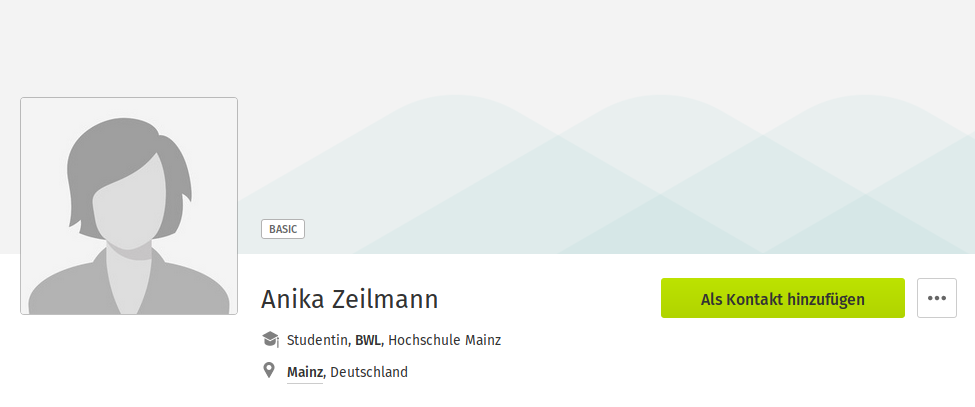
\includegraphics[ scale=0.2]{bilder/XING_profil.png}
		\caption{Profil von der Webseite XING}
		\label{img:XING}
	\end{figure}

	\subsection{LinkedIn}
	LinkedIn ist das weltweit größte soziale Netzwerk für Berufstätige mit mehreren Millionen Mitgliedern. Es vernetzt berufliche Kontakte der ganzen Welt und stellt ebenfalls Möglichkeiten zum Schutz der Privatsphäre zu Verfügung. \cite{WasIstLinkedIn}
	\begin{figure}[H]
		\centering
		
\includegraphics[ scale=0.2]{bilder/LinkedIn_profil.png}
		\caption{Profilkarte von der Webseite LinkedIn}
		\label{img:Linkedin}
	\end{figure}

		\subsection{Fupa}
		Die Webseite Fupa stellt ein regionales Fußballportal dar, welches zur Berichterstattung des Amateurfußballs vorhanden ist. Allerdings werden nicht nur Berichte sondern auch aussagekräftige Spielerprofile zur Verfügung gestellt.\cite{WasIstFUPA} Außer dem verzeichnet FuPa eine Mitgliederzahl von über 200.000.\cite{FuPaMitglieder}\\
		Das Bild \ref{img:FuPa} zeigt ein Spielerprofil, wie es auf dieser Webseite angezeigt wird. Allerdings kann sich die Vollständigkeit eines Profils variieren.
		\begin{figure}[H]
			\centering
			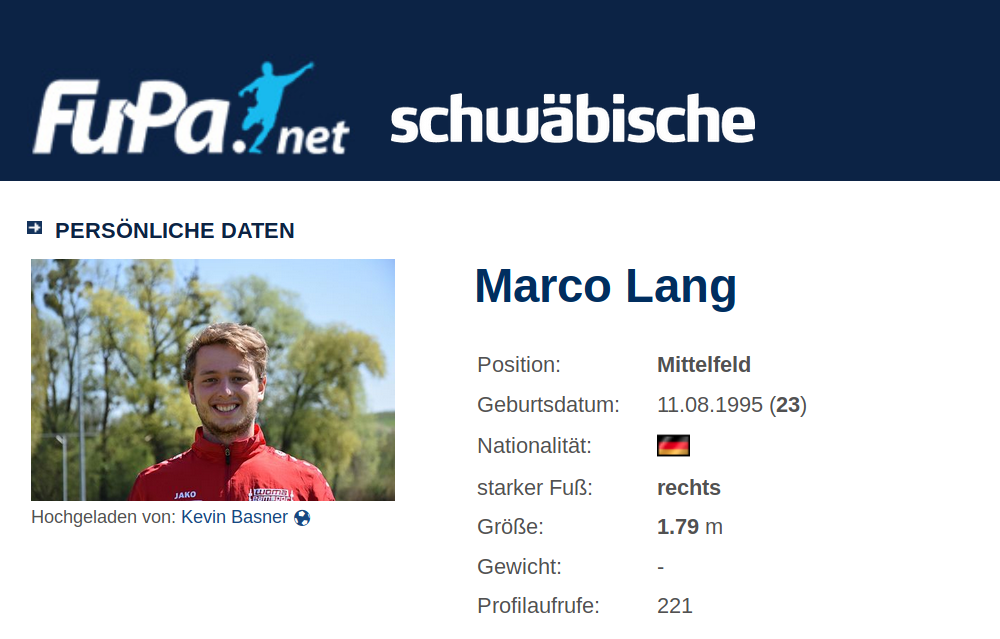
\includegraphics[ scale=0.2]{bilder/fupa_screenshot.png}
			\caption{Spielerprofil von der Webseite FuPa}
			\label{img:FuPa}
		\end{figure}
		%TODO wie viele Mitglieder hat fupa?
	
	\section{Konzept für die Erstellung einer Phishing-Mail}
	Die Generierung einer realen Phishing-Mail benötigt eine korrekte E-Mail-Adresse der Zielperson und einen sinnvollen Inhalt, der die gewonnenen Informationen verwendet.
	\subsection{E-Mail-Adresse Generierung}
		\subsubsection{Algorithmus entwickeln zum generieren}
		Es kann ein Algorithmus entwickelt werden, der mögliche E-Mail-Adressen aus den gewonnen Daten generiert. Dies ist durch die Kombination aus Vorname, Nachname, Geburtsjahr und den bekanntesten E-Mail-Providern realisierbar. Dabei entsteht ein Adresspool, von dem jede einzelne E-Mail-Adresse auf Validität geprüft werden muss.\\
		\subsubsection{Automatisierbare OSINT-Tools verwenden}
		Für die Generierung der E-Mail-Adressen kann ein kostenloses OSINT-Tools von Michael Bazzel verwendet werden. Diese Tool ermöglicht es, die gewonnenen Informationen über eine Formular einzugeben. Anschließend werden draus mögliche E-Mail-Adressen generiert. Auch hier entsteht ein Adresspool, bei dem die E-Mail-Adressen auf Validität geprüft werden. Zu dem bringt das Tool eine weitere Funktion mit sich. Es wird automatisch nach Einträgen, der generierten E-Mail-Adressen, im Internet gesucht und angezeigt. \cite{EmailAssumptions}

	\subsection{E-Mail Inhalt}
		\subsubsection{E-Mail-Muster erstellen}
		Die zu erstellenden E-Mail-Muster entsprechen hier kategorisierten Lückentexten. Abhängig von den gefundenen Daten, wird ein Lückentext ausgewählt und anschließend mit den Daten an den passenden Stellen ergänzt.\\
		Die Lückentexte werden so kategorisiert, dass für jede gefundene Information ein passender Lückentext vorhanden ist. Eine denkbare Unterteilung wären die Kategorien Privat und Geschäftlich.
		\subsubsection{Text aus Fragmenten erzeugen}
		Bei dieser Methode besteht der E-Mail-Text aus zusammengesetzten Fragmenten. Dafür wird zu jeder gefundenen Information ein Fragment erstellt und anschließend werden alle Fragmente zu einem Text zusammengefügt.
		
		
		


%Kapitel des Hauptteils

\chapter{Bewertung der Lösungsideen anhand der Anforderung}  %Name des Kapitels
\label{cha:BewertungLösungsideenAnhandAnforderung} %Label des Kapitels

\section{Bewertung der OSINT-Methoden für eine ausgewählte Person}
Es gibt zwei verschiedene Methoden um OSINT zu betreiben. Die erste Lösungsidee beschreibt die Verwendung von einem öffentlich frei zugänglichen OSINT-Tool. Dieses Tool bietet zahlreiche Möglichkeiten um eine Person beziehungsweise Daten über eine Person zu finden. Allerdings ist es auf dieser Webseite nicht möglich, ein Profil zur gesuchten Person anzugeben. Es kann nur eine begrenzte Anzahl an Daten über ein Formular eingegeben werden. Des Weiteren wird bei einer Suche ausschließlich nach dem Namen oder einer E-Mail gesucht. Das Suchergebnis ist dadurch kein vollständiges Personenprofil, es werden lediglich Verweise auf weitere Webseiten mit möglichen Einträgen angezeigt.\\
Im Gegensatz zu diesem Tool nutzt der eigene Algorithmus alle im Vorfeld bekannten Daten für eine Suche. Es wird nicht auf Webseiten mit möglichen Informationen verwiesen, sondern Profile der Zielpersonen erstellt. Durch die Verwendung eines eigenen Algorithmus kann die Suche an die Anforderungen beliebig angepasst werden. Zusätzlich besteht die Möglichkeit zur Optimierung der Suche durch die Verwendung der Techniken aus \cite{Bazzell}.
\section{Bewertung der Methoden zur Erstellung einer Phishing-Mail}
	\subsection{Generierung der E-Mail-Adressen}
	Ein bereitgestelltes OSINT-Tool ist ein komplettes und funktionsfähiges System. Dadurch wird kein zusätzlicher Aufwand für die Entwicklung eines Algorithmus benötigt. Lediglich die Automatisierung des Tools muss erstellt werden. Allerdings kann nicht jede Information über die Person zur Generierung der E-Mail-Adresse genutzt werden. Dies ist ein großer Nachteil. Die Wahrscheinlichkeit, dass sich die richtige Adresse unter den erzeugten befindet, sinkt dadurch.\\
	Bei einem eigenen Algorithmus fließen dagegen alle Information mit in die Generierung einer E-Mail-Adresse ein. Beispielsweise auch das Geburtsjahr einer Zielperson, was bei dem OSINT-Tool \cite{EmailAssumptions} nicht verwendet wird. Jedoch können die vom OSINT-Tool generierten Adressen, als Anregung und Ideengeber für den eigenen Algorithmus dienen.\\
	Für die erfolgreiche Simulation eines Phishing-Mail-Angriffes wird die korrekte E-Mail-Adresse benötigt. Aus diesem Grund wird der eigene Algorithmus verwendet. Dadurch wird die Wahrscheinlichkeit erhöht, dass sich die korrekte Mail-Adresse in dem Pool befindet.
	%TODO Anzahl der Möglichen E-Mail-adressen ausrechenen
	
	\subsection{E-Mail-Text}
	Der Inhalt einer E-Mail ist sehr wichtig für die Glaubwürdigkeit einer Phishing-Mail. Es ist die einzige Möglichkeit, bei der ein Angreifer mit dem Opfer kommunizieren kann. Aus diesem Grund ist es von Bedeutung, dass der E-Mail-Text Sinn ergibt und eine korrekte Grammatik enthält. Bei der dynamischen Texterzeugung mit der Fragment-basierten Methode \ref{subsubsec:EMailTextFragment} kann die Grammatik und der Zusammenhang des Textes zu einer Problematik führen. Durch die Verkettung von verschiedensten Fragmenten könnte ein Text erzeugt werden, welcher keinen sinnvollen Zusammenhang hat. Allerdings muss hierbei nicht für jede Kombination aus gewonnen Daten ein vollständiges Fragment-Muster erstellt werden. Wogegen bei der Verwendung von fertigen Lückentexten ein Muster für jede Kombination aus gewonnen Daten vorhanden sein muss. Dennoch ist die Glaubwürdigkeit durch einen sinnvollen E-Mail-Text höher. Das hat den Grund, dass ein Opfer dadurch vermutet, dass dieser Text von einem Menschen verfasst wurde. Somit werden die vollständigen E-Mail-Muster umgesetzt.


	

%%Kapitel des Hauptteils

\chapter{Lösungsideen}  %Name des Kapitels
\label{cha:Lösungsideen} %Label des Kapitels
Für die Umsetzung der im Kapitel \ref{sec:Zielsetzung} definierten Ziele, werden folgende Lösungsideen vorgeschlagen.

\section{Programmiersprache}
Python
%TODO Warum Python? Antworten finden

\section{Informationsbeschaffung}
Für die Eingabe von Suchdaten, besteht für beide Informationsbeschaffungen die Möglichkeit eine Grafische-Bedienoberfläche oder eine Konsolen-Eingabe zu verwenden.
	\subsection{Informationsbeschaffung von bestimmten/ausgewählten Personen}
		
		\subsubsection{Suche nach Informationen}
		\label{sec:Suche nach Information}
		{\bf Idee 1} \textit{Die Art der Suche wird anhand den eingegebenen Daten angepasst.}\\\\
		Abhängig von der Anzahl und Art der Daten die vom Programm-Anwender eingeben wurden, wird die Art beziehungsweise die Reihenfolge der Suche variiert. Die nachfolgenden Fälle sollen diesen Ansatz verdeutlichen.\\\\
		\textit{Fall 1: Vorname, Nachname, Ort wird eingeben:}\\
		In diesem Fall wird mit Hilfe der Suchmaschine von Google nach Information gesucht. Die von Google vorgeschlagenen Seiten werden analysiert, interpretiert und gespeichert. Dadurch können weitere Informationen gewonnen werden. Wenn Benutzernamen von anderen Webseiten wie Instagram, Facebook oder ähnliches vorgeschlagen wird, kann somit die Suche speziell auf der entsprechenden Seite erweitert werden.\\\\
		\textit{Fall 2: Benutzername einer Webseite(Facebook,Instagram,usw.) wird eingeben:}\\
		Hier kann zuallererst auf der entsprechenden Webseite nach Informationen zu dem angegebenen Benutzername gesucht werden. Möglicherweise werden dadurch zusätzliche Daten herausgefunden, die bei der weiteren Suche von Vorteil wären.\\
		Nachdem die Webseite nach dem Nutzernamen durchsucht und ausgewertet wurde, kann nun mit herkömmlichen Suchmaschinen die Suche erweitert werden.\\\\
		{\bf Idee 2} \textit{Es wird unabhängig von den eingegebenen Daten direkt mit einer Suchmaschine nach Informationen gesucht.}\\\\
		Man verwendet ausschließlich die herkömmlichen Suchmaschinen und geht anhand den vorgeschlagenen Links auf die Suche nach Informationen.\\\\
		{\bf Idee 3} \textit{Es wird nur auf ausgewählten Webseiten nach Informationen gesucht}\\\\
		Verschiedenste Webseiten durchsuchen. Ideen dafür sind Facebook, FuPa, Instagram, Xing, LinkedIn, Google und Twitter.\\
		
		\subsubsection{Wann handelt es sich um die gleiche Person?}
		Bei jeder einzelnen Suchvariante, besteht die Herausforderung darin, zu erkennen, wann es sich um die gesuchte Person handelt. Für diese Problematik werden folgende Lösungsideen vorgeschlagen.\\
		
		{\bf Lösungsidee 1} \textit{Die Art der Suche wird anhand den eingegebenen Daten angepasst.}\\
		Diese Lösung entspricht dem Ansatz 1 von Kapitel \ref{sec:Suche nach Information}. Die Suche kann dadurch verfeinert werden und die Anzahl der fehlerhaften Vorschläge wird geringer. Dadurch wird die Wahrscheinlichkeit höher, dass es sich um die richtige Person handelt.\\\\
		{\bf Lösungsidee 2} \textit{Bei keiner perfekten Übereinstimmung wird die Suche erweitert}\\
		Hier kann das Such erweitert werden, indem auf Verbindungen der Zielperson eingegangen wird. Das heißt bekannte Facebook-Freunden, FuPa-Teammitglieder, oder Xing-Arbeitskollegen gesucht können ebenfalls durchsucht werden.\\
		
		{\bf Lösungsidee 3} \textit{Profilbilder können verglichen werden}\\ Entweder mit Bilderkennungssoftware oder Googl-Bildersuche\\
		
		{\bf Lösungsidee 4} \textit{Die Personen-Suche mit Hilfe von korrekten Suchbefehlen verfeinern.}\\
		In dem Buch "'Open Source Intelligence Techniques"' \cite{Bazzell}, werden Suchbefehle aufgezeigt, mit denen die Suche mit bekannter Suchmaschinen verbessert und verfeinert werden kann. Auch bei dieser Lösungsidee wird die Wahrscheinlichkeit erhöht, dass es sich um die gesuchte Person handelt. %TODO Buchzitat in bib einfügen
		
	\subsection{Informationsbeschaffung von einer großen Menge unbestimmter Personen}
	Webseiten mit großen Menge von Daten, ausgenommen von den bekannten Social Media Seiten, sind das Fußballportal FuPa, Xing und LinkedIn.
	
\section{Analyse und Speicherung der Information}
	\subsection{Textanalyse}
	Die Textanalyse wird nur bei der Suche einer bestimmten Person benötigt. Die  zweite Suchfunktion wird hartkodiert und benötigt dadurch keine Textanalyse, da der Aufbau der Webseite im voraus bekannt ist. Das bedeutet, dass das Programm genau weiß wo welche Information auf der Webseite steht. Beispielsweise befindet das Geburtsjahr bei der Seite von dem Fußballportal FuPa immer an der gleichen Position einer Tabelle.\\
	Dies ist bei der ersten Suchfunktion allerdings nicht möglich. Es können verschiedenste Arten von Webseiten vorgeschlagen werden. Aus diesem Grund muss das Programm "'clever"' sein und die wichtigen Daten aus der Seite herausfiltern können. Dazu gibt es folgende Lösungsideen.\\
	
	{\bf Idee 1} \textit{Textanalyse mit Hilfe von Python NTLK.}\\
	Mit dem\textit{Natural Language Toolkit} ist es möglich, den vorhandenen Webseitentext zu analysieren. Zu beginn können sogenannte "'stopwords"' aus dem vorgegebenen Text herausgefiltert werden. Stopwords sind Wörter die sehr oft auftreten und keinen großen Informationsgewinn mit sich bringen. Beispiele dafür sind ist, ein, einer, usw. Dadurch verringert sich die Anzahl der gesamten Wörter im Text. Anschließend können Funktionen wie das Zählen des Vorkommens einzelner Wörter angewendet werden, um einen Überblick von dem Text zu bekommen. Des Weiteren kann der Text in Fragmente zerlegt werden um weitere Informationen über den Inhalt zu erlangen. Abschließend können die analysierten Wörter bzw. Fragmente nach Schlüsselbegriffen durchsucht werden.\\
	
	{\bf Idee 2} \textit{Textanalyse indem nach Schlüsselwörtern gesucht wird.}\\
	Es kann ein Algorithmus entwickelt werden, der nach Schlüsselwörtern in einer Webseite sucht. Hierfür wäre es denkbar, Datenbanken bzw Wortsammlungen zu erstellen, die die zu suchenden Schlüsselwörter beinhalten. Mit diesen Datenbanken kann nun die Webseite nach den Schlüsselwörter durchsucht,analysiert und interpretiert werden. Die Datenbanken werden mit Hilfe von bekannter Listen im Internet befüllt. Beispiele hierfür wären eine aktuelle Liste aller Hochschulen in Deutschland, Berufsbezeichnungen, Studiengänge, Hobbys, Städte, etc...\\
	
	{\bf Idee 3} \textit{Textanalyse mit Hilfe Machine Learning}\\
	Möglicherweise irgendeine Python bib.
	
	Scikit\\
	
	{\bf Idee 4} \textit{Mit Hilfe von NLTK Rake den Text interpretieren}\\
	Rake hat die Aufgabe, einen Text mit vielen Wörten auf eine geringe Anzahl von Schlüsselwörter zu reduzieren und dadurch kann möglicherweise der Inhalt des Textes erkannt werden ohne ihn komplett gelesen zu haben.
	
	\subsection{Speicherung der Information}
	Für die Suche einzelner Person, kann ein erweiterbares Personen-Objekt erstellt werden.\\
	Für die Informationsbeschaffung von vielen unbekannten Personen, könnte eine SQL-Datenbank erstellt werden. Ein weiterer Idee wäre, eine Datei anzulegen, bei der alle Personen gut strukturiert gespeichert werden können. Möglichkeiten dafür wären die Dateiformate CSV und TXT.%TODO ist TXT Dateiformat wirklich eine gute Möglichkeit

\section{Generierung der E-Mail-Adressen}
Es kann das opensource tool von intelligencetechniques mit Hilfe eines automatisierten Webbrowsers verwendet werden. Algorithmus entwickeln, der alle möglichen Mail-Adressen aus den Daten Vorname, Nachname, Geburtsjahr und den bekanntesten Mail-Providern erzeugt.

\section{Erstellung der E-Mail-Muster}
Die Muster können in zwei große Kategorien unterteilt werden. Es gibt einen privaten und geschäftlichen Teil. Der private Teil hat weiter Unterteilungen wie Familie, Hobby/Interessen.
\section{Erzeugung der Phishing-Mail}
		% des Hauptteils
%
%Kapitel des Hauptteils

\chapter{Auswahl der Lösung anhand den Anforderungen}  %Name des Kapitels
\label{cha:Auswahl der Lösung anhand Anforderungen} %Label des Kapitels
\section{Programmiersprache/ GUI}
Python
\section{Informationsbeschaffung von ausgewählten Personen}
	
\section{Informationsbeschaffung von einer großen Menge unbestimmter Personen}
Einfachheitshalber wird CSV verwendet.
	\subsection{Auslesen der Webseite}
	Diese Suchfunktion wird \textit{hartkodiert} und benötigt dadurch keine Textanalyse, da der Aufbau der Webseite im voraus bekannt ist. Das bedeutet, dass das Programm genau weiß wo welche Information auf einer Webseite steht. Beispielsweise befindet sich das Geburtsjahr einer Person, auf der Seite von dem Fußballportal "'FuPa"', immer an der gleichen Position einer Tabelle. Dies bringt den Vorteil mit sich, dass der Text nicht analysiert werden muss und das Programm genau weiß, was mit diesen Daten gemacht werden muss.
\section{Generierung der E-Mail-Adressen}
%TODO Anzahl der Möglichen E-Mail-adressen ausrechenen

\section{Erstellung der E-Mail-Muster}

\section{Erzeugung der Phishing-Mail}		% sollten hier in der
%Kapitel der Umsetzung

\chapter{OSINT einer ausgewählten Person}  %Name des Kapitels
\label{cha:Informationsbeschaffung einer ausgewählten Person} %Label des Kapitels

\section{Auswahl der Programmiersprache}
Damit das Programm anhand den Lösungsideen umgesetzt werden kann, ist der erste Schritt die Auswahl der Programmiersprache.\\
Hierbei wird keine Anforderung an die Geschwindigkeit der Sprache gestellt, da beim web scraping das Internet den zeitlichen Engpass darstellt. Allerdings wäre es von Vorteil wenn bereits entwickelte Bibliotheken für das OSINT vorhanden sind. Die Eingabe der Information für die Suche kann über eine Konsole oder über eine graphische Benutzeroberfläche möglich sein.\\
Als mögliche Programmiersprachen zählen Python, Ruby, C++.\\
Für web-basierende Anwendung eignet sich eine dynamische Programmsprache.
Im Gegensatz zu Python und Ruby zählt C++ nicht zur Familie der dynamischen Programmiersprachen und fällt aus diesem Grund als mögliche Lösung heraus. \\
Python und Ruby können beide Webseiten, die JavaScript zum rendern benötigen, laden. Dies ist mit Hilfe eines automatisierten Webbrowsers möglich. Des Weiteren lässt sich die Anwendung durch beide Sprachen, entsprechend den Anforderungen entwickeln. Es kann sowohl eine Oberflächenanwendung als auch eine Konsolenanwendung programmiert werden. Zusätzlich bringen beide Sprachen Module mit sich, um das Pojekt mit den vorgegebenen Zielen umzusetzen. Somit haben beide Programmiersprachen die Voraussetzungen für die Entwicklung der Anwendung. Allerdings bietet Python in diesem Bereich eine große Community und eignet sich sehr gut für die Bearbeitung von linguistischen Daten. \cite{bird2009natural}
Aus diesen Gründen wird die zu erstellende Anwendung mit der Programmiersprache Python entwickelt.
	
\section{Methoden zur Suche nach einer Person im Internet}
\label{sec:Suche nach Information}
Die Art der Personensuche wird abhängig von den eingegeben Daten  variiert. Das heißt, dass die eingegebenen Daten über die Zielperson vor der Suche analysiert werden und dementsprechend angepasst wird. Nachstehen werden zwei grundsätzliche Methoden für die Art der Personensuche beschrieben.

	\subsection{Personensuche mit Hilfe einer Suchmaschine}
	\label{subsubsec:PersonensucheMitHilfevonSuchmaschine}
	Hier wird mit Hilfe einer Suchmaschine nach Informationen gesucht. Mögliche Suchmaschinen sind die von Google und Bing. Allerdings muss nicht für jede Suche eine Suchmaschine verwendet werden. Die nachfolgenden Fälle sollen diesen Ansatz verdeutlichen.
	
	Im Fall, dass der Vorname, Nachname und Wohnort der gesuchten Person eingegeben wird, kann mit Hilfe der festgelegten Suchmaschine nach Information gesucht werden. Die von der Suchmaschine vorgeschlagenen Seiten werden anschließend analysiert, ausgelesen und gespeichert. Dadurch können weitere Informationen gewonnen werden. Falls Benutzernamen von anderen Webseiten wie Instagram, Facebook oder ähnliches vorgeschlagen werden, kann somit die Suche mit diesen Daten speziell auf den entsprechenden Seiten erweitert werden.
	
	Ein weiterer Fall beschreibt das Szenario, wenn ein Benutzername der gesuchten Person in das Programm eingegeben wird. Hierbei handelt es sich um einen Benutzernamen von Social-Media-Webseiten wie Facebook, Instagram, LinkedIn, et cetera. \\
	Zuallererst, wird hier nach Einträgen auf der entsprechende Webseite zu dem angegebenen Benutzername gesucht. Dadurch können zusätzliche Daten herausgefunden werden. Diese sind bei der weiteren Suche von Vorteil.\\
	Sobald die Webseite mit Hilfe des Nutzernamens durchsucht und ausgewertet wurde, kann die Suche mit einer Suchmaschine und den gewonnen Daten erweitert werden.
	
	\subsection{Personensuche auf festgelegten Webseiten}
	\label{subsubsec:PersonensucheohneSuchmaschine}
	Unabhängig von den eingegebenen Daten, wird eine festgesetzte Anzahl von Webseiten durchsucht. Als potentielle Kandidaten-Webseiten eigenen sich die Social-Media-Seiten wie Facebook, Instagram, Twitter, LinkedIn, et cetera. Diese Art der Personensuche arbeitet allerdings ohne die Verwendung einer Suchmaschine.
	
\section{Bewertung der Methoden zur Personensuche}
Um möglichst viele Informationen über eine Person im Internet zu finden, bietet die Personensuche mit der Verwendung einer Suchmaschine die beste Lösung. Es wird anstatt ausschließlich festgelegten Seiten das ganze Internet durchsucht. Dadurch können wesentlich mehr individuelle Einträge gefunden werden. Des Weiteren wird keine Logik zur Suche nach Einträgen im Internet benötigt, da lediglich den vorgeschlagenen Suchergebnissen gefolgt werden kann.\\
Allerdings muss beachtet werden, dass Benutzer bei verschiedensten Social-Media-Seiten auswählen können, ob das Benutzerprofil von einer Suchmaschine gefunden werden kann oder nicht. Bekannte Webseiten die diese Einstellungsmöglichkeiten unterstützen sind XING und LinkedIn. Aus diesem Grund, werden zu Beginn der Suche die Social-Media-Seiten durchsucht. Dadurch können vor der Google-Suche zusätzliche Informationen herausgefunden werden, die für das später OSINT von Vorteil sind. Falls sich eine Social-Media-Seite unter den Google-Suchergebnissen befindet, kann diese nachträglich ebenfalls durchsucht werden.

	\subsection{Auswahl der Suchmaschine}
	Laut Expertenaussage sucht Bing tiefgreifender nach Information auf Social Media Seiten wie Facebook, Twitter und LinkedIn. Allerdings finden nur 3,5\% aller Suchanfragen in Deutschland über Bing statt. Im Gegensatz dazu hat Google einen Marktanteil von 91,2\% in Deutschland. Diese Zahlen sprechen eindeutig für Google. Durch die höhere Anzahl von Suchanfragen, können mehr Daten erfasst und die Ergebnislisten besser gerankt werden. Dies hat zu Folge, dass Bing bei einer konkreten Suche schlechter abschneidet. \cite{Suchmaschinen}
	Grundsätzlich stellt die Verwendung von zwei Suchmaschinen die beste Lösung dar, da die Wahrscheinlichkeit für einen Suchtreffer erhöht wird. Dennoch wird in dieser Arbeit ausschließlich die Suchmaschine von Google verwendet, da sie gegenüber dem Konkurrenten keine Nachteile hat. Selbst die detailliertere Suche auf Sozialen Netzwerken, bringt bei der hier verwendeten Personensuche keinen großen Vorteil für Bing. Das heißt, durch die Analyse der Suchergebnisse, wird erkannt ob sich die bekannten Social Media Webseiten darunter befinden. Falls diese es nicht tun, wird die Suche auf den entsprechenden Sozialen Netzwerken erweitert.
	 	
\section{Umsetzung: Personensuche mit Hilfe der Google-Suchmaschine im Internet}
Die Suchmaschine von Google wird für die Personensuche im Internet verwendet. Gesucht wird nach den eingegebenen Daten, welche über die Konsole eingelesen werden.

	\subsection{Eingabe der bekannten Daten}
	Es besteht die Möglichkeit den \textbf{Vorname, Nachname, Wohnort, Arbeitgeber, Instagram Benutzername, Facebook Benutzername, Twitter Benutzername, E-Mail-Adresse}, und das genaue beziehungsweise geschätzte \textbf{Geburtsjahr} der gesuchten Person über eine Konsole einzugeben. Falls der genaue Jahrgang der Zielperson nicht bekannt ist, kann ein geschätztes Geburtsjahr eingetragen werden. Dies kann später bei der Identifizierung der gesuchten Person hilfreich sein.\\
	Zu Beginn werden alle Personen-Variablen mit einem leeren String initialisiert. Das bedeutet, alle Variablen, zu denen keine Information eingegeben wurde, enthalten einen leeren String.
	
		\subsubsection{Verarbeitung der Daten}
		Im ersten Schritt wird kontrolliert, welche Informationen vom Progamm-Nutzer eingegeben wurden. Der Vorname und Nachname sind nicht ausreichend für die Suche. Es wird mindestens ein weiteres Attribute benötigt. Dagegen ist der Benutzernamen von Instagram und Twitter sowie die E-Mail-Adresse einzigartig. Dadurch kann mit einem dieser Attribute gesucht werden.\\
		Bei der Eingabe des Wohnortes, kann dieser vor der Suche mit der entsprechenden Wortsammlung verglichen werden. Falls sich der Wohnort nicht in der Datenbank befindet, wird er nachträglich ergänzt. Für die Personenerkennung ist es wichtig, dass sich der korrekt Wohnort in der Datenbank befindet.\\
		Daraufhin werden mit diesen Eingaben Kombinationen für die Suche und die URL-Generierung erstellt. Mögliche Such-Kombinationen für erfolgreiche Ergebnisse sind:
		
		\textit{Vorname, Nachname, Wohnort;}\\
		\textit{Vorname, Nachname, Geburtsjahr;}\\
		\textit{Vorname, Nachname, Institution;}\\
		\textit{Vorname, Nachname, Wohnort, Geburtsjahr;}\\
		\textit{Vorname, Nachname, Wohnort, Institution;}\\
		\textit{Benutzername einer Social-Media-Seite;}
		
		
		Die Kombination aus vielen oder allen Daten ist ebenfalls eine mögliche Option. Allerdings wird dadurch oft kein Ergebnis gefunden, da nicht zur jeder Information ein Eintrag im Internet besteht.\\
		Sobald die Kombinationen aus den Daten bekannt sind, werden die Such-URLs für die Google-Suchmaschine generiert.
		\subsection{Generierung der Google-Such-URLs}
			\subsubsection{Aufbau eines URLs}
			\label{subsec:AufbauURL}
			Ein Uniform Resource Locator, kurz URL, lokalisiert eine Ressource, indem eine abstrakte Identifikation der Lokalisierung verwendet wird. Dabei wird ein URL grundsätzlich im folgenden Format angegeben.\cite{RFC1738}
			
			$<scheme>:<scheme-specific-part>$ \cite{RFC1738}
			
			Das Schema gleicht hierbei meist dem verwendeten Protokoll wie HTTP oder FTP. Der Doppelpunkt stellt die Trennung zum Schema-spezifischen Teil dar. Ein Beispiel für ein HTTP-URL-Aufbau ist im Folgenden definiert.\cite{RFC1738}
			
			$http://<host>:<port>/<path>?<searchpart>$\cite{RFC1738}
			
			Hier wird das Protokoll HTTP als Schema verwendet, wobei sich der Aufbau bei der Verwendung des HTTPS-Protokolls kaum unterscheidet. Lediglich das Schema und der Port verändert sich.\\
			Für den <host> kann der FQDN oder die IP-Adresse des Hostrechners eingetragen werden. Wenn der Port nicht angegeben wird, ist der Standardport voreingestellt. Bei HTTP wäre dies Port 80 und bei HTTPS Port 443. Der <path> stellt ein HTTP-Selektor dar und ist mit einem Fragezeichen von der Suchzeichenkette getrennt.\cite{RFC1738}\\ %TODO FQDN in Abkürzungsverzeichnis	
			Im Bereich des <searchpart> lassen sich URL-Parameter einfügen um Informationen an die entsprechende Webseite mitzugeben. Die Parameter bestehen aus einem Schlüssel und aus einem Wert, welche durch ein Gleichheitszeichen getrennt werden. Um mehrere Parameter hinzuzufügen und zu kombinieren wird das kaufmännische Und-Zeichen verwendet.\cite{GoogleURL}\\
			Ein URL für die Google-Suche von \textit{Max Mustermann} ist in dem folgenden Beispiel gegeben.
			
			$https://www.google.com/search?q=Max+Mustermann$
			%TODO Möglicherweise zeichnung mit Beschriftung wie bei wikipedia
			
			Allerdings können URLs nur mit ASCII-Zeichen erzeugt und versendet werden. Aus diesem Grund müssen Zeichen die nicht im ASCII vorkommen, in ein gültiges Format umgewandelt werden. Dies wird realisiert, indem die URL-Kodierung das nicht enthaltende ASCII-Zeichen durch ein "'\%"', gefolgt von zwei Hexadezimalen Ziffern, ersetzt. Beispielsweise repräsentiert "'\%20"' ein Leerzeichen und "'\%22"' ein Anführungszeichen. \cite{HTMLURL} \\
			
			\subsubsection{Erstellen der Such-URLs}
			Dieser Absatz beschreibt die Erstellung der Such-URLs für Google, mit dem Wissen aus Kapitel \ref{subsec:AufbauURL}.\\
			Für jede genannte Kombination aus den eingegebenen Daten werden Link-Muster erzeugt. Diese entsprechen einem Lückentext. Sobald die entsprechenden Muster ausgewählt wurden, werden die Lücken mit den Daten befüllt. Dadurch wird eine Liste mit einer variierende Menge von Suchlinks erstellt. Diese Liste wird anschließende von dem Web Crawler verwendet um die Suche zu starten.
			Ein URL für die Suche nach Information auf beliebigen Webseiten wird wie folgt dargestellt.
			
			\textit{https://www.google.com/search?q=\%22Max+Mustermann\%22+\%22Weingarten\%22}
			
			Wenn allerdings der Benutzername einer Social-Media-Seite bekannt ist, werden zwei unterschiedliche URLs verwendet. Mit Hilfe des ersten URLs, wird speziell nach Einträgen auf der entsprechenden Webseite gesucht. Dazu kann der Operator "'site"' verwendet werden. Dieser beschränkt die Suchergebnisse soweit, dass die vorgeschlagenen Einträge ausschließlich auf einer festgelegten Webseite vorkommen. Das folgende Beispiel beschreibt die Suche nach dem Benutzer "'Mustermann"' auf der Webseite "'Instagram.com"'. Dabei ersetzt die ASCII-Zeichenkette "'\%3A"' den Doppelpunkt. \cite{HTMLURL}
			
			\textit{https://www.google.com/search?q=site\%3Ainstagram.com+\%22Mustermann\%22}
			
			Der zweite URL wird für eine Social-Media-Suche verwendet. Bei dieser Suche werden Social-Media-Seiten nach Einträgen durchsucht. Dafür wird kein zusätzlicher Operator benötigt. Es wird lediglich ein @-Zeichen, welches mit der Zeichenkette "'\%40"' dargestellt wird, vor dem zu suchenden Wort eingefügt. Die Social-Media-Suche nach dem Benutzernamen "'Mustermann"' sieht folgendermaßen aus.\cite{SocialMediaSearch}
			
			\textit{https://www.google.de/search?q=\%40Mustermann}
			
			\subsubsection{Optimierung der Such-URLs}
			\label{subsubsec:URLOptimieren}
			Um die Suchergebnisse von Google zu verbessern, können die Suchbegriffe in Anführungszeichen gesetzt werden. Dadurch wird eine Phrasensuche gestartet, die nach einer Zeichenfolge sucht. Das bedeutet, es wird ausschließlich nach diesen Zeichenfolgen gesucht und nicht nach einer Abwandlung. Ein Beispiel hierfür ist die Suche nach "'Mike Bazzell"'. Wenn diese Suche ohne Anführungszeichen durchgeführt wird, werden zusätzlich Webseiten vorgeschlagen die den Namen Mike Bazzell anstatt Micheal Bazzell beinhalten. Diese erweiterte Suche kann dazu führen, dass unzählige Webseiten vorgeschlagen werden, die nicht unbedingt was mit dem Thema der Suchbegriffe zu tun hat. Um dem vorzubeugen können Anführungszeichen verwendet werden, welche die Anzahl der Suchergebnisse um einen sehr großen Teil verringern. \cite{Bazzell}\\
			Für die Suche nach \textbf{Marco Lang} werden ungefähr \textbf{96.400.000} Ergebnisse mit Hilfe der Google-Suchmaschine gefunden. Wird die Suche mit den Anführungszeichen verfeinert indem nach \textbf{"'Marco"' "'Lang"'} gesucht wird, werden etwa \textbf{55.600.000} Ergebnisse gefunden. Allerdings werden hier Webseiten vorgeschlagen, welche die Wörter "'Marco"' und "'Lang"' beinhalten, jedoch müssen diese nicht direkt nebeneinander und auch nicht in der Reihenfolge vorkommen. Es wäre Möglich, dass bei dieser Suche, Webseite mit Verweisen auf die Namen "'Marco Mustermann"' und "'Max Lang"' beinhaltet. Aus diesem Grund kann nach \textbf{"'Marco Lang"'} gegoogelt werden. Dadurch wird die Anzahl der Suchergebnisse auf \textbf{45.500} Ergebnisse reduziert. Der Grund für die starke Reduzierung ist, dass ausschließlich die Webseiten vorgeschlagen werden, die den kompletten String "'Marco Lang"' beinhalten. Für eine weitere Optimierung der Ergebnisse, wird der Wohnort hinzugefügt, wie in dem Beispiel \textbf{"'Marco Lang"' "'Tettnang"'}. Dadurch werden die Suchvorschläge auf lediglich \textbf{95} Ergebnisse reduziert. Die URL zu dieser optimierten Suche lautet: 
			
			\textit{https://www.google.com/search?q=\%22Marco+Lang\%22+\%22Tettnang\%22}
			
			Nicht nur die Reduzierung der Suchergebnisse, sondern auch das herausfiltern von unerwünschten Webseiten hat einen positiven Effekt auf die zu erstellende Anwendung, da die vorgeschlagenen Seiten in den folgenden Schritten analysiert werden müssen. Das bedeutet, dass jede unerwünschte Seite die allein durch die Suche herausgefiltert werden kann, einen großen Laufzeitvorteil mit sich bringt. 
			
			
		
		\subsection{Mit welcher Bibliothek werden Serveranfragen umgesetzt?}
		Damit eine Person im Internet gesucht werden kann, muss das Programm in der Lage sein, Anfragen an einen Server zu versenden und die dazugehörigen Antwort zu empfangen. \\
		Im Folgenden werden drei Möglichkeiten beschrieben, um Anfragen an einen Server zu versenden. Zum einen ist das die Python Request-Bibliothek, welche sich optimal für HTTP-Anfragen eignet.\cite{WebScraping} Zum anderen bietet sich die Verwendung eines automatisierten Webbrowsers an, was mit Hilfe der Selenium Python API realisierbar ist.\cite{lawson2015web} Über diese API ist es möglich auf alle Funktionen des Selenium WebDrivers zuzugreifen.\cite{SeleniumWithPython} Eine Alternative dazu, ist das Python Framework Scrapy, welches zum Crawlen von Webseiten und Extrahieren von Daten verwendet werden kann.\cite{Scrapy} Die letzte Möglichkeit stellt die  Scrapy Middleware Scrapy-Selenium dar.\cite{scrapy-selenium} Dadurch wird die Kommunikation von Scrapy und Selenium ermöglicht.
		
		Für komplizierte Anfragen an einen Server eignet sich die Request-Bibliothek von Python sehr gut. Der Umgang mit Cookies, Header und vielem mehr ist sehr einfach gestaltet. Auch die Generierung des Such-URLs wird von dieser Bibliothek übernommen. Des Weiteren hat Requests einen großen Laufzeit-Vorteil gegenüber dem automatisierten Webbrowser und kann HTTP-Fehlermeldungen empfangen. Allerdings lässt sich mit der Request-Bibliothek keine Javascript-Seite auslesen.\\
		Wenn das Framework Scrapy standardmäßig verwendet wird, können ebenfalls keine Javascript-Seiten ausgelesen werden. Doch in Scrapy lässt sich ein automatisierter Webbrowser einfügen, mit welchem das Auslesen von Javascript-Webseiten möglich ist. Zusätzlich lässt sich mit Scrapy ein effektiver Web Crawler und Web Scraper entwickeln, was für die nächsten Schritte ein erheblicher Vorteil ist.\\
		Aus den erläuternden Gründen, wird das Framework Scrapy mit der Verbindung eines automatisierten Webbrowsers für die Personensuche verwendet. Der automatisierte Webbrowser muss in dem Framework implementiert werden, da auf bestimmte Webseiten mit Javascript direkt zugegriffen wird. Infolgedessen wird die Middelware Scrapy-Selenium verwendet, da sie die eine kompakte Möglichkeit bietet, den automatisierten Webbrowser in Scrapy zu implementieren. Durch diese Kombination aus Scrapy und dem Selenium WebDriver, lassen sich Javascript-Seiten problemlos auslesen. \\
		Zusätzlich zu diesem Framework wird ein unabhängiger Selenium-Wedriver implementiert. Dieser wird für den Umgang mit den Social-Media-Seiten benötigt, da auf diesen Seiten ein Login vollzogen werden muss. Das hat den Vorteil, dass die Anmeldung in der Session gespeichert wird. Somit muss bei einem erneuten Zugriff auf die selbe Seite keine neue Anmeldung vollzogen werden.
	
		\subsection{Web Crawler erstellen}
		%TODO Muss Scrapy und Selenium erklärt werden?

		Nachdem der Selenium WebDriver in das Scrapy Framework implementiert wurde, kann mit dem crawling begonnen werden. Der Web Crawler hat die Aufgabe ausgewählte Social-Media-Seiten zu durchstöbern und den von Google vorgeschlagenen Webseiten zu folgen. Wie in Bild \ref{img:AufbauWebCrawler} gezeigt, werden zuerst die Informationen über die Zielperson eingelesen. Anschließend werden die Social-Media-Seiten behandelt, wodurch weitere Informationen über die Person gefunden werden können. Die bekannten Informationen über die gesuchte Person, werden zur Generierung der Google-Such-Links verwendet. Mit diesen Links und der Hilfe von der Google-Suchmaschine, werden Webseiten gesucht, die mögliche Inhalte betreffend der Zielperson enthalten. Im nächsten Schritt wird die Google-Webseite mit den Suchergebnissen analysiert und ausgelesen. Dadurch können die URLs für die entsprechenden Webseiten gewonnen werden. Diesen URLs wird anschließend gefolgt, um Informationen über die Zielperson zu gewinnen.\\
		
		\begin{figure}[H]
			\centering
			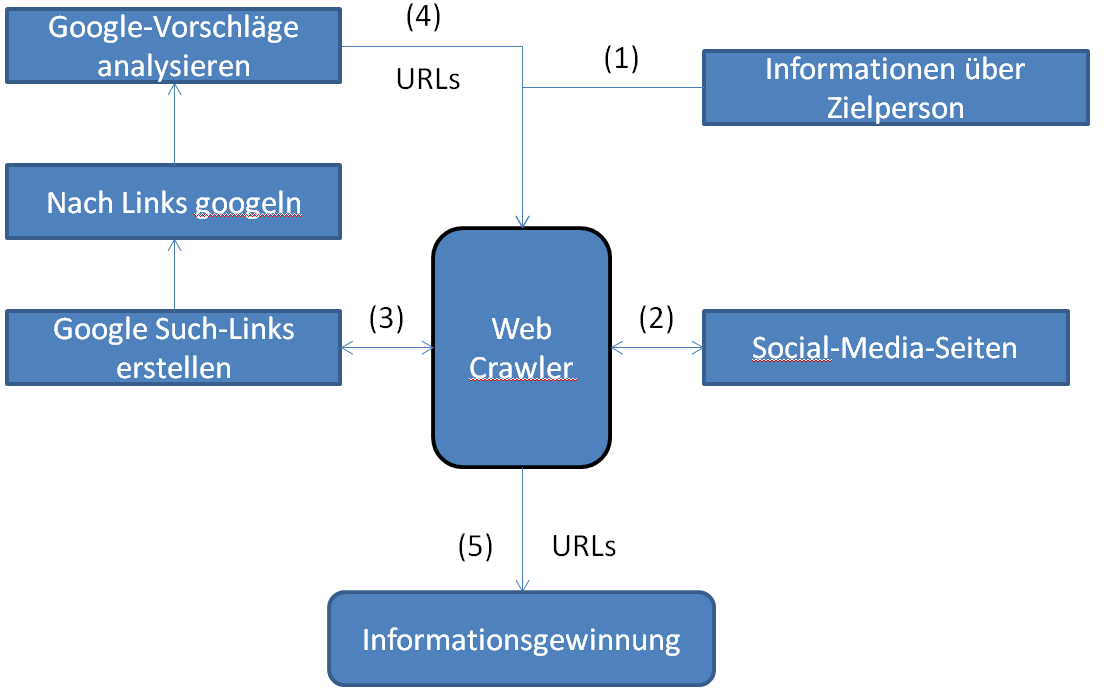
\includegraphics[ scale=0.5]{bilder/webcrawler.PNG}
			\caption{Aufbau des Web Crawlers}
			\label{img:AufbauWebCrawler}
		\end{figure}
		%TODO Bild ohne roten Linien einfügen
		
			\subsubsection{Social-Media-Seiten}
			\label{subsubsec:SocialMediaSeiten}
			Zu den verwendeten Social-Media-Webseiten gehören Instagram, Facebook, Twitter, Xing und LinkedIn. Für diese Webseiten werden Fake-Accounts und ein eigener Selenium WebDriver erstellt. Dieser automatisierte Webbrowser ist ausschließlich für die Social-Media-Seiten zuständig. Damit vollständige Profile angezeigt werden können, loggt sich dieser automatisch ein. Die gewonnen Informationen werden dem Profil der gesuchten Person hinzugefügt und zusätzlich für die Google-Suche verwendet.\\
			Es kann passieren, dass ausschließlich der Benutzername von einer Person bekannt ist. Weiter Attribute wie Vorname, Nachname und Wohnort sind nicht bekannt. In dem Fall, kann mit einem einzigartigen Benutzername nach diesen Attributen auf der entsprechenden Webseite gesucht werden. Jedoch verwendet nur Instagram und Twitter ein einmaligen Benutzernamen. Aus diesem Grund kann die erweiterte Suche nur auf diesen beiden Plattformen umgesetzt werden.
			
			\textbf{Login-Formulare}\\
			Der Selenium WebDriver muss sich nicht bei jeder Social-Medi-Webseite einloggen. Zu beginn wird kontrolliert, zu welcher Plattform ein Benutzername eingegeben wurde. Dazu gibt es bei dieser Anwendung die Möglichkeit einen Facebook-, Instagram- oder Twitter-Benutzername einzugeben. Je nach Eingabe meldet sich der Browser auf den entsprechenden Seiten an. Auf den Seiten Xing und LinkedIn wird sich standardmäßig  angemeldet. Das hat den Grund, dass diese beiden Seiten immer durchsucht werden sollen. \\
			Bei der Umsetzung wird im ersten Schritt die Login-Seite der entsprechenden Plattform angefordert. Die Antwort wird mit Hilfe der BeautifulSoup-Bibliothek nach dem HTML-Tag <input> durchsucht. Allerdings hat nicht jede Webseite den komplett identischen Aufbau. Das bedeutet, dass sich bei diesen Tags die Attribute unterscheiden können. Aus diesem Grund muss nach der Angeforderten-Webseite die Suche der <input>-Tags unterschieden werden.\\
			Die Anmeldung von Instagram, Facebook und LinkedIn sind nahezu identisch. Hier können die zwei gesuchten <input>-Felder mit Hilfe des Attributs \textit{type} identifiziert und gefunden werden. Bei der Twitter-Login-Seite muss anstatt dem \textit{type} nach dem Attribute \textit{class} gesucht werden. Andernfalls findet der Browser keine interaktiven Elemente.\\
			Zum übertragen der Benutzernamen und Passwörter, benötigt der Selenium WebDriver ein Element mit eindeutigem Attribut zur Referenzierung. Dafür dient bei Instragram, LinkedIn und Facebook das vorher gefundene Element mit dem Attribute "'id"'. Bei Twitter ist das dass Attribut "'class[0]"' und bei Xing "'name"'.
			 
			\textbf{Instagram}\\
			Instagram und Twitter verwenden beide einen einzigartigen Benutzername. Dies ist ein riesigen Vorteil für die Identifikation einer Person, wenn der Benutzername bekannt ist. Allerdings ist es ebenfalls möglich eine Person mit ihrem offiziellen Namen zu suchen und zu finden.\\
			Im Fall, dass der Instagram-Benutzername eingegeben wurde, wird die dazugehörige Profilseite angezeigt und nach Informationen durchsucht. Im nächsten Schritt dienen die vorgeschlagenen Freunde, welche in Beziehung zu diesem Profil stehen, als weitere Informationsquelle. Das bedeutet, dass diese Kontakte ebenfalls durchsucht werden. Bei Übereinstimmungen wie zum Beispiel der selben Universität, kann später eine glaubwürdige Phishing-Mail generiert werden.\\
			Falls sich jedoch eine Instagram-Seite unter den Google-Vorschlägen befindet, und die Übereinstimmung des Profils mit der Zielperson nicht klar ist, können die Vorgeschlagenen Kontakte für die Identifizierung der Zielperson genutzt werden. So wird beispielsweise erkannt, wenn ein Freunden aus der selben Stadt vorgeschlagen werd, dass es sich um die gesuchte Person handeln kann. Diese Methode erzielt kein sicheres Ergebnis. Jedoch kann die Wahrscheinlichkeit erhöht werden, dass es sich um die richtige Person handelt.\\
			Die Profilseite wird mit dem folgenden Link \textit{https://www.instagram.com/username/} angefordert. Weitere Seiten und Einträge der gesuchten Person, unabhängig von der Profilseite,können mit dem Suchbefehl \textbf{site:instagram.com "'username"' \\ -site:instagram.com/username} angezeigt werden. \cite{Bazzell} In der Anwendung wird dies mit dem folgenden URL umgesetzt.
					
			\textit{https://www.google.com/search?q=site\%3Ainstagram.com+\%22username\%22+-site\\
				\%3Ainstagram.com\%2Fusername\&oq=site\%3Ainstagram.com+\%22username\%22+-site\\
				\%3Ainstagram.com\%2Fusername}
			
			Die dazugehörigen Suchergebnisse werden anschließend gleich den normalen Google-Suchergebnissen behandelt.
			
			\textbf{Twitter}\\
			Auf der Webseite Twitter wird ausschließlich die Profilseite nach Informationen durchsucht. Dies ist mit dem Link \textbf{https://twitter.com/username} möglich.
			
			\textbf{Facebook}\\
			Facebook bietet ein großes Potential um OSINT zu betreiben. Allerdings hat Facebook optimal Algorithmen zur Erkennung von automatisierten Crawlern entwickelt. Aus diesem Grund wurde das Fake-Konto nach wenigen Versuchen gesperrt. Das hat zu Folge, dass auf dieser Plattform nur begrenzt gesucht werden kann, da keine Anmeldung vorgenommen wird. Um das Konto zu entsperren müssten eine Kopie des Ausweises, ein Bild mit erkennbarem Gesicht und eine Handynummer an Facebook übermittelt werden.\\
			Aus diesen Gründen wird Facebook nur dann und ohne Anmeldung verwendet, wenn sich ein Vorschlag unter den Google-Suchergebnissen befindet.

			\textbf{LinkedIn und XING}\\
			LinkedIn und XING bieten eine optimale Informationsquelle bezüglich der schulischen und beruflichen Laufbahn der Zielperson. Allerdings gibt es hier keinen einzigartigen Benutzernamen. Demzufolgem, wird eine Person mit dem vollen Namen und dem aktuellen Wohnort gesucht. Dabei wird auf LinkedIn ein Filter angewendet, bei dem ausschließlich Personen aus Deutschland angezeigt werden. Wenn genau eine Person vorgeschlagen wird, wird dieses gefundene Personenprofil durchsucht. Bei einer Mehrzahl von gefunden Personen werden diese nicht auf Informationen durchsucht, da keine Identifikation möglich ist.\\
			Die Personensuche bei LinkedIn, mit angwandtem Filter, wird mit dem URL\\ \textit{https://www.linkedin.com/search/results/people/?facetGeoRegion=\%5B\%22de\%3A0\%22\%5D\\
				\&keywords=vorname\%20nachname\%20wohnort\&origin=FACETED\_SEARCH} dargetellt. \\
			Bei Xing sieht der Such-URL wie folgt aus.\\			
			\textit{https://www.xing.com/search/old/members?hdr=1\&keywords=vorname+nachname++wohnort}
			
			
			\subsubsection{Webseite mit den Suchergebnissen von Google analysieren}
			Zur Analyse der Webseite mit den Suchergebnissen von Google, wird der Seitenquelltext benötigt. Mit Hilfe des Quelltextes, können  die entsprechenden Links erkannt werden. Der Seitenquelltext wird mit Hilfe der BeautifulSoup-Bibliothek angezeigt.\\
			Das Bild \ref{img:GoogleSuchergebnis} stellt ein Suchergebnis von Google dar. Der dazugehörige Quelltext befindet sich im Bild \ref{img:GoogleSeitenquelltext}.
			\begin{figure}[H]
				\centering
				
\includegraphics[ scale=0.65]{bilder/Google-Suchergebnis1.png}
				\caption{Google-Suchergebnis}
				\label{img:GoogleSuchergebnis}
			\end{figure}
			Im Ausschnitt des Seitenquelltextes \ref{img:GoogleSeitenquelltext} ist zu sehen, dass der <div>-Container mit der Klasse "'g"' einen Hyperlink enthält. URLs oder Links werden mit dem HTML-Tag <a> dargestellt. Dieser Link wird für die Suche benötigt. Deswegen wird genau nach diesem Link gesucht.\\
			Da der <div>-Container bei jedem Suchergebnis identisch ist, kann bei jedem Ergebnis nach dem entsprechenden <div>-Container gesucht werden. Anschließend kann der erste Link in diesem <div>-Tag ausgelesen werden. Dies wird mit Hilfe der BeautifulSoup-Bibliothek umgesetzt.\\ %TODO DIE oder DER URL
			Um zu erkennen, ob mehrere Seiten mit Suchergebnissen existieren, wird nach bestimmten Hyperlinks gesucht. Diese Links werden über das Attribute "'class"' identifiziert. Mit Hilfe der BeautifulSoup-Bibliothek wird nach dem Klassennamen "'fl"' gesucht. Falls weiter Seiten mit Suchergebnissen vorhanden sind, werden die dazugehörigen Links in einer Liste gespeichert. Anschließend wird ihnen gefolgt und die neue Seite wird nach weiteren URLs durchsucht.\\
			%TODO sollen wirklich mehrere Seiten durchsucht werden???\\
			
			\begin{figure}[H]
				\centering
				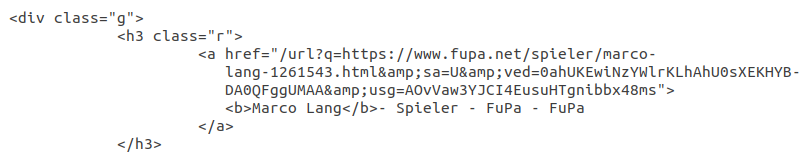
\includegraphics[ scale=0.6]{bilder/code_googleResults.png}
				\caption{Ausschnitt des Quelltextes von einem einem Google-Suchergebnis}
				\label{img:GoogleSeitenquelltext}
			\end{figure}
			%TODO lstlisting anstatt bild, dafür html als sprache verwenden
			

\section{Methoden zum Erkennen von wichtigen Informationen auf einer Webseite}
\label{subsec:ErkennenVonInformation}
Bei der Suche nach einer ausgewählten Person können verschiedenste Arten von Webseiten gefunden werden. Aus diesem Grund muss das Programm eine gewisse Intelligenz mit sich bringen um die wichtigsten Daten aus einer Seite herauszufiltern. Dabei ist es nicht möglich eine Hartkodierung zu verwenden, um festgelegte Bereiche einer Webseite auszulesen, da jede Webseite eine individuelle Struktur hat.\\
Die Grundidee zur Lösung diese Problems ist die Analyse des vorliegenden Webseiten-Textes. Eine Methode zur Textanalyse ist die automatisierte Schlüsselwort-Gewinnung. Hierbei wird die HTML-Seite zu einem verwendbaren Text formatiert, wobei alle Sonderzeichen herausgefiltert werden. Für die E-Mail-Erkennung wird der unformatierte Text verwendet, da Sonderzeichen wie "'."' und "'@"'  dabei von Nöten sind. Im nächsten Schritt werden Schlüsselwörter aus dem formatierten Webseitentext generiert. Möglichkeiten zur automatisierten Schlüsselwortgenerierung sind die Verfahren RAKE \ref{sec:RAKE} und die Automatic Keyword Extraction mit NLP \ref{sec:Automatic Keyword Extraction}, welche im Laufe dieser Arbeit detailliert beschrieben werden.\\
Nachdem die Schlüsselwörter generiert und in Listen gespeichert wurden, werden Wortsammlung erstellt. Diese Wortsammlungen sind Listen, welche aussagekräftige Schlüsselwörter enthalten und nach Themen kategorisiert sind. Beispiele für den Inhalt der Listen sind alle Hochschulen und Universitäten in Deutschland, Berufsbezeichnungen und Tätigkeiten, Studiengänge, Hobbybezeichnungen und alle Städte und Gemeinden in Deutschland.\\
Mit diesen Wortsammlungen kann nun die Liste mit den bereits generierten Schlüsselwörtern aus dem Webseitentext verglichen werden. Bei einer Übereinstimmung eines Schlüsselwortes wird das Wort mit der entsprechenden Kategorie vorgemerkt und später in die verwendete Speicherstruktur eingetragen. \\
Die Wortsammlungen werden mit Hilfe von bekannten Listen im Internet eigenständig befüllt. Als Informationsquelle dienen alle öffentlich frei zugänglichen Listen, die hilfreiche Informationen enthalten.

	\subsection{RAKE}
	\label{sec:RAKE}
	RAKE steht für \textit{Rapid Automatic Keyword Extraction} und stellt eine sehr effiziente Methode zur Schlüsselwortgenerierung dar. Die Funktion von RAKE basiert darin, dass Schlüsselwörter mehrere Wörter mit inhaltlicher Relevanz enthalten, allerdings selten Stoppwörter und Sonderzeichen.\cite{rose2010automatic}\\
	Als Stoppwörter werden Wörter bezeichnet, die sehr oft auftreten und keinen großen Informationsgewinn mit sich bringen. Beispiele dafür sind \textit{und}, \textit{weil}, \textit{der} oder \textit{als}.\cite{Stopwords}\\
	
	\begin{figure}[h!]
		\fbox{\parbox{\linewidth}{In einer jungen Wissenschaft wie der Informatik mit ihrer Vielschichtigkeit und ihrer unüberschaubaren Anwendungsvielfalt ist man oftmals noch bestrebt, eine Charakterisierung des Wesens dieser Wissenschaft und Gemeinsamkeiten und Abgrenzungen zu anderen Wissenschaften zu finden. Etablierte Wissenschaften haben es da leichter, sei es, dass sie es aufgegeben haben, sich zu definieren, oder sei es, dass ihre Struktur und ihre Inhalte allgemein bekannt sind.}}
		\caption{Beispieltext}
		\label{fig:text}
	\end{figure}
	%TODO QUELLE für Beispieltext einfügen.
	
	Zu Beginn wird der zu analysierende Text, hier der Beispieltext in  Bild \ref{fig:text}, durch einen Worttrenner in ein Array, bestehen aus möglichen Schlüsselwörtern, aufgeteilt. Das erzeugte Array wird anschließend in Sequenzen von zusammenhängenden Wörtern unterteilt. Dabei erhalten die Wörter in einer Sequenz die gleiche Position und Reihenfolge wie im Ursprungstext und dienen gemeinsam als Kandidatenschlüsselwort.\cite{rose2010automatic}\\		
	Nachdem die möglichen Schlüsselwörter identifiziert sind, wird für jeden einzelnen Kandidaten ein Score ausgerechnet. Dieser besteht aus dem Quotient des Grades $deg(w)$ und der Häufigkeit des Vorkommens eines Wortes innerhalb der Kandidaten $freq(w)$. Daraus ergibt sich die Formel:
	\begin{center}
		$deg(w)/freq(w) $
	\end{center}	
	
	Dabei beschreibt der Grad eines Wortes, dass gemeinsame Auftreten mit sich selbst und anderen Schlüsselwörtern. In der Tabelle \ref{tab:Co-occurance} ist der Grad für jedes Wort ablesbar, indem die Einträge in der entsprechenden Reihe summiert werden. Beispielsweise Beträgt der Grad des Wortes \textit{"'Wissenschaft"'} den Wert \textit{3}. Dies ergibt sich aus der Rechnung:
	\begin{center}
		$2 + 1 = 3$
	\end{center}
	Das Wort \textit{"'Wissenschaft"'} kommt hier selbst zweimal in dem Kandidaten-Array vor und davon einmal in Verbindung mit dem Worten "'jungen"'.\\
	Die Häufigkeit des Vorkommens eines Wortes lässt sich ebenfalls in der Tabelle \ref{tab:Co-occurance} ablesen. Allerdings muss hier in der Reihe und Spalte des jeweiligen Wortes nachgeschaut werden. Für das Wort \textit{"'Wissenschaft"'} beträgt die Häufigkeit des Vorkommens den Wert \textit{3}.\\
	Zusammenfassend kann gesagt werden, dass \textit{deg(w)} die Kandidaten bevorzugt, welche oft und in langen Schlüsselwörtern, die mehrere Wörter enthalten, vorkommen. Dies bedeutet, dass beispielsweise \textit{deg(etabliert)} eine höhere Bewertung als \textit{deg(informatik)} bekommt, obwohl beide Wörter gleich oft im Text vorkommen. Dagegen wird bei \textit{freq(w)}, ausschließlich die Häufigkeit des Vorkommens bewertet. Bei der Formel \textit{deg(w)/freq(w)} werden die Wörter bevorzugt, welche überwiegend in langen Kandidatenwörtern vorkommen. Diese Formel bietet dadurch einen guten Mittelweg zur Schlüsselwortgewinnung. Ein Beispiel dafür sind die Wörter \textit{"'Wissenschaften} und \textit{"'allgemein"'}. Hier ist der Quotient von \textit{deg(allgemein)/freq(allgemein)} höher als von \textit{deg(Wissenschaften)/freq(Wissenschaften)}, obwohl die Häufigkeit des Wortes \textit{"'Wissenschaften"'} höher und der Grad gleich hoch ist. \cite{rose2010automatic}
	
	Durch das genannte Verfahren und der Formel \textit{deg(w)/freq(w)} für die Bewertung, ergeben sich die im Bild \ref{fig:SchlüsselwörterMitScore} befindenden Kandidaten mit den dazugehörigem Endbewertungen. \cite{rose2010automatic}
	
	\begin{center}
		\begin{table}[h!]
			\scriptsize
			\begin{tabular}{*{24}{l|}}				
				\rotatebox[origin=c]{90}{} 
				&\rotatebox[origin=c]{90}{wissenschaften} &\rotatebox[origin=c]{90}{wissenschaft} &\rotatebox[origin=c]{90}{sei} &\rotatebox[origin=c]{90}{etablierte} &\rotatebox[origin=c]{90}{informatik} &\rotatebox[origin=c]{90}{aufgegeben} &\rotatebox[origin=c]{90}{gemeinsamkeiten} &\rotatebox[origin=c]{90}{oftmals} &\rotatebox[origin=c]{90}{charakterisierung} &\rotatebox[origin=c]{90}{jungen} &\rotatebox[origin=c]{90}{inhalte} &\rotatebox[origin=c]{90}{allgemein} &\rotatebox[origin=c]{90}{bekannt} &\rotatebox[origin=c]{90}{struktur} &\rotatebox[origin=c]{90}{wesens} &\rotatebox[origin=c]{90}{bestrebt} &\rotatebox[origin=c]{90}{unüberschaubaren} &\rotatebox[origin=c]{90}{anwendungsvielfalt} &\rotatebox[origin=c]{90}{definieren} &\rotatebox[origin=c]{90}{abgrenzungen}
				&\rotatebox[origin=c]{90}{leichter}
				&\rotatebox[origin=c]{90}{finden}
				&\rotatebox[origin=c]{90}{vielschichtigkeit}\\
				\hline
				wissenschaften & 2 & & & 1 & & & & & & & & & & & & & & & & & & &\\
				\hline
				wissenschaft & & 2 & & & & & & & & 1 & & & & & & & & & & & & & \\
				\hline
				sei & & & 1 & & & & & & & & & & & & & & & & & & & &	\\
				\hline
				etablierte & 1 & & &1 & & & & & & & & & & & & & & & & & & &	\\
				\hline
				informatik & & & & &1 & & & & & & & & & & & & & & & & & & \\
				\hline
				aufgegeben & & & & & &1 & & & & & & & & & & & & & & & & &	\\
				\hline
				gemeinsamkeiten & & & & & & & 1& & & & & & & & & & & & & & & &	\\
				\hline
				oftmals & & & & & & & & 1& & & & & & & & & & & & & & &\\
				\hline
				charakterisierung & & & & & & & & & 1& & & & & & & & & & & & & & \\
				\hline
				jungen & & 1 & & & & & & & & 1 & & & & & & & & & & & & &	\\
				\hline
				inhalte & & & & & & & & & & & 1 & 1 & 1 & & & & & & & & & &	\\
				\hline
				allgemein & & & & & & & & & & & 1 & 1 & 1 & & & & & & & & & & \\
				\hline
				bekannt & & & & & & & & & & & 1 & 1 & 1 & & & & & & & & & &	\\
				\hline
				struktur & & & & & & & & & & & & & &1 & & & & & & & & &	\\
				\hline
				wesens & & & & & & & & & & & & & & &1 & & & & & & & &\\
				\hline
				bestrebt & & & & & & & & & & & & & & & & 1& & & & & & & \\
				\hline
				unüberschaubaren & & & & & & & & & & & & & & & & & 1 & 1 & & & & &	\\
				\hline
				anwendungsvielfalt & & & & & & & & & & & & & & & & & 1 & 1 & & & & &	\\
				\hline
				definieren & & & & & & & & & & & & & & & & & & & 1 & & & & \\
				\hline
				abgrenzungen & & & & & & & & & & & & & & & & & & & & 1 & & &	\\
				\hline
				leichter & & & & & & & & & & & & & & & & & & & & & 1 & &	\\
				\hline
				finden & & & & & & & & & & & & & & & & & & & & & & 1 & \\
				\hline
				vielschichtigkeit & & & & & & & & & & & & & & & & & & & & & & & 1	\\
				\hline
			\end{tabular}
			\label{tab:Co-occurance}
			\caption{Co-occurance}
		\end{table}
	\end{center}
	
	\begin{figure}[h!]
		\fbox{\parbox{\linewidth}{ inhalte allgemein bekannt (9.0), unüberschaubaren anwendungsvielfalt (4.0), jungen wissenschaft(3.5), etablierte wissenschaften (3.5), wissenschaften (1.5), wissenschaft (1.5), wesens (1.0), vielschichtigkeit (1.0), struktur (1.0), sei (1.0), oftmals (1.0), leichter (1.0), informatik (1.0), gemeinsamkeiten (1.0), finden (1.0), definieren (1.0), dass (1.0), charakterisierung (1.0), bestrebt (1.0), aufgegeben (1.0), abgrenzungen (1.0)}}
		\caption{Schlüsselwörter mit zugehörigem Score}
		\label{fig:SchlüsselwörterMitScore}
	\end{figure}
	\FloatBarrier

	\subsection{Automatic Keyword Extraction mit NLP}
	\label{sec:Automatic Keyword Extraction}
	Bei dieser Methode wird der vorliegende Text in die einzelnen Wörter unterteilt. Dabei wird eine Liste mit potentiellen Schlüsselwörtern erstellt, in der \textit{Stoppwörter} und Sonderzeichen herausgefiltert werden. Bei den Schlüsselwörtern handelt es sich nicht ausschließlich um ein Wort sondern auch um Wortsequenzen. Sogenannte N-Gramme bestehen aus einer festgelegten Anzahl von Wörtern. Dies hat den Vorteil, dass nicht nur Schlüsselwörter bestehend aus einem Wort erstellt werden können, sondern auch Schlüsselwörter mit Fragmenten eines Textes. Diese Art von Schlüsselwort wird benötigt um Informationen wie \textit{Hochschule Ravensburg-Weingarten} herauszulesen.\\
	Erweiternd kann die Anzahl der Schlüsselwörter mit dem Verfahren von Stemming reduziert werden. Durch die Verwendung von ergänzende Regeln wie, eine Mindestanzahl von Buchstaben in einem Wort, können die Schlüsselwörter weiter begrenzen.

 

\section{Bewertung: Herausfiltern von wichtigen Informationen auf einer Webseite}
RAKE stellt eine fertige Methode dar, um Schlüsselwörter, die den Inhalt eines Textes in kurz wiedergeben, zu erstellen. Dabei hat ein Anwender kaum Möglichkeiten eigene Implementierungen vorzunehmen, da vieles vorgegeben ist. In der zu erstellenden Anwendung soll jedoch nicht der Inhalt eines Textes in Schlüsselwörter zusammengefasst werden, sondern es wird nach informationsreichen Wörtern gesucht. Aus diesem Grund ist jedes einzelne Wort aus dem Webseiten-Text von Bedeutung. Dies spricht gegen RAKE, da es nur die selbst errechnenden Favoriten-Schlüsselwörter zur Verfügung stellt. Dadurch werden viele Wörter nicht in Betracht gezogen oder für weiterführende Bearbeitungen nicht bereitgestellt. Darüber hinaus ist die Berechnung eines Scores für diese Anwendung nicht notwendig.\\
Die Methode zur automatisierten Schlüsselwortgenerierung mit NLP bringt dagegen ein eigene Implementationsmöglichkeit mit sich. Das bedeutet, es kann selbst festgelegt werden, aus wie vielen Wörtern die Schlüsselwörter bestehen sollen. Des Weiteren wird jedes einzelne Wort in Betracht gezogen und verwendet.\\ Die Suche nach einer E-Mail-Adresse im Text lässt sich bei beiden Methoden hinzufügen. Jedoch wird aus den eben genannten Vorteilen, die Information mit Hilfe der Methode zur automatisierten Schlüsselwortgewinnung mit NLP herausgefiltert.


\section{Implementierung der Methode zum Herausfiltern von wichtigen Informationen auf einer Webseite}
	\subsection{Text formatieren}
	\label{subsec:TextFormatieren}
	Bevor die Schlüsselwörter generiert werden können, muss der Text in ein verwertbares Format umgewandelt werden. Aus diesem Grund wird der Seitenquelltext zuallererst mit Hilfe des Python-Skripts html2text zu einem ASCII Plaintext umgewandelt.\cite{html2text} Anschließend werden Zeilenumbrüche und Sonderzeichen aus diesem Text herausgefiltert. Einzelne Wörter und Zahlen die weniger als 2 Zeichen beinhalten, werden ebenfalls aussortiert. Nachdem der Text in ein verwertbares Format umgewandelt wurde, kann mit der Umsetzung für die automatisierte Schlüsselwortgenerierung mit NLP begonnen werden.
	\subsection{Automatic Keyword Extraction mit NLP}
	\label{subsec:AutomaticKeywordExtractionNLP}
	Durch das \textit{Natural Language Toolkit} (NLTK) von Pyhton ist es möglich, den vorhandenen Webseitentext zu analysieren.\\
	Zu Beginn wird der vorhandene Text in einzelne Wörter zerlegt und in eine Liste gespeichert. Aus diesen Wörtern werden die \textit{stopwords} der deutschen als auch der englischen Sprache herausgefiltert. Dadurch verringert sich die Anzahl der gesamten Wörter im Text um einen sehr großen Teil. \\
	Im nächsten Schritt werden die N-Gramme erstellt. Es werden nicht nur Bigramme sondern auch Trigramme, Tetragramme, Pentragramme und Hexagramme benötigt, damit vollständige Universitätsnamen und Firmennamen aus dem Text erkannt werden können. Alle erzeugten N-Gramme werden der eben erstellten Liste hinzugefügt. Diese Schlüsselwortliste wird später mit den Wortsammlungen verglichen.
	%TODO möglicherweise Code erklären
		\subsubsection{N-Gramme erstellen}
		%TODO Umsetzung und Beispiele aufzeigen
		
	\subsection{Wortsammlungen erstellen}
	Die Ausführlichkeit der Wortsammlungen ist sehr wichtig für das Projekt, da die Informationsgewinnung abhängig von diesen Listen ist. Das bedeutet, umso besser diese Datenbanken erstellt werden, umso mehr Informationen können gewonnen werden.
	
		\subsubsection{Erstellung der Wortsammlungen}	
		Eine Wortsammlung ist eine CSV-Datei die manuell erstellt und befüllt wird. Es gibt eine Wortsammlung mit allen Universität- und Hochschulnamen, Städten und Gemeinden in Deutschland, Vereinskürzel, Bezeichnungen für Tätigkeiten und Hobbys sowie einer Liste mit den bekanntesten Firmennamen. 
		%TODO möglicherweise ausführlicher schreiben mit Lösungsidee,Bewertung,...
		\subsubsection{Wie werden sie am effektivsten verglichen?}
		Es gibt keine Methode die den Vergleich der Schlüsselwörter mit den Wörtern der Datenbanken verbessern kann, da jedes einzelne Schlüsselwort mit jedem einzelnen Wort aus der Datenbank verglichen werden muss. Suchalgorithmen
		
	\subsection{Geburtsjahr herausfinden}
	Das Geburtsjahr ist für die Generierung der E-Mail wichtig. Viele Personen verwenden eine Kombination aus dem bürgerlichen Namen und dem Geburtsjahr als lokalen Teil der E-Mail-Adresse. Aus diesem Grund wird speziell nach dem Geburtsjahr in den generierten Schlüsselwörtern aus Kapitel \ref{subsec:AutomaticKeywordExtractionNLP} gesucht.\\
	Dazu wird eine Suche nach einer vierstelligen Zahl, welche größer als 1900 und kleiner-gleich 2019 ist, durchgeführt. Beim Fund einer Zahl, werden  fünfzehn Schlüsselwörter vor und hinter der vermutlichen Jahreszahl kontrolliert. Falls dabei das Wort "'Geburtsdatum"', "'Alter"', "'geboren"', "'Geburtsort"', "'Geburtstag"', "'born"', oder "'birth"' vorkommt, wird das entsprechende Jahr als Geburtsjahr der Zielperson festgelegt. Die Implementierung zur Erkennung eines Geburtsjahrs ist in Listing \ref{lst:AlgoYearOfBirth} dargestellt.\\
	
	\begin{lstlisting}[caption=Geburtsdatum herauslesen,label={lst:AlgoYearOfBirth}]
	regex_string = "(geburtsdatum)|(alter)|(geboren)|(geburtsort)|	
					(geburtstag)|(born)|(birth)"
	for year in all_years_in_text:
		vistited_elements = 0
		max_number_of_visited_elements = 15
		#  to get all occurrences of this year
		occurrences = [i for i, x in enumerate(keywords) if x == year]
		for position_of_year in occurrences:
			while (position_of_year+vistited_elements) < len(keywords)-1 and
				vistited_elements <= max_number_of_visited_elements and
				position_of_year is not -1:
				index_behind = position_of_year+ vistited_elements
				index_front = position_of_year - vistited_elements
				if re.match(r""+regex_string, keywords[index_behind]):
					print("Behind: Geburtsjahr wurde gefunden", year)
					return year
				elif re.match(r""+regex_string, keywords[index_front]):
					print("Front: Geburtsjahr wurde gefunden", year)
					return year
				vistited_elements += 1
	return -1
	\end{lstlisting} 
	\subsection{E-Mail-Adressen erkennen und herauslesen}
	Zu beginn wird der unformatierte Webseitentext in Textfragmente zerlegt. Getrennt wird der Text bei einem Leerzeichen. Anschließend werden die erzeugten Fragmente mit einem regulären Ausdruck nach einer gültigen E-Mail-Adresse durchsucht. Bei einer Übereinstimmung des regulären Ausdrucks, wird der korrekte Teilstring, somit die E-Mail-Adresse, ausgelesen. Der Algorithmus zu diesem Vorgang ist in Listing \ref{lst:AlgoEMail} aufgezeigt.\\
	
	\begin{lstlisting}[caption=E-Mail-Adressen herrauslesen,label={lst:AlgoEMail}]
	for fragment in email_words:
		mail_regex = re.search('(.*((@)|(\(at\))).*\.(de|com|net)).*',
		fragment)
		if mail_regex:
			print("Email found:", mail_regex.group(1))
	\end{lstlisting}   

	Es werden nur die E-Mail-Adressen herausgesucht, welche einen Bezug zur Zielperson haben. Aus diesem Grund wird der lokale Teil aller gefunden Adressen mit dem Vor-und Nachnamen der Zielperson vergleichen. Mit Hilfe der difflib von Python, lassen sich diese beide Sequenzen vergleichen und es wird ein prozentuale Übereinstimmung berechnet. Zur Differenzierung, ob eine E-Mailadresse eine Verbindung zum Opfer hat oder nicht wird eine Prozent-Grenze bestimmt. Die Grenze wurde aus den Ergebnissen von zahlreichen Tests auf die Zahl 0,4 \% festgelegt. Das folgende Beispiel soll die Methode zur Erkennung von korrekten E-Mail-Adressen verdeutlichen.\\
	In diesem Beispiel heißt die Person "'Max Mustermann"' und es werden zwei E-Mail-Adresse gefunden. Die erste Adresse lautet \textit{MusterMax@gmail.com} und die zweite \textit{MartaFrau@gmx.de}. Im ersten Schritt wird der Name "'Max Mustermann"' zu einem String "'maxmustermann"' umgewandelt. Im nächsten Schritt werden die lokalen Namen aus den E-Mail-Adressen herausgelesen und gleichzeitig in Kleinbuchstaben umgewandelt. In diesem Fall wäre das "'mustermax"' und "'martafrau"'. Anschließend werden die lokalen Namen der E-Mail-Adressen mit dem erzeugten Namensstring der Zielperson vergleichen. Dabei erreicht die lokale Namen \textit{mustermax} eine prozentuale Übereinstimmung von 0,73 \% mit dem Namensstring und \textit{martafrau} 0,27 \%. Da die Prozent-Grenze bei 0,4 \% beträgt, wird die zweite E-Mail-Adresse verworfen.
		
\section{Methoden zum Erkennen einer Person}
\label{sec:WannhandeltessichumdiegesuchtePerson}
Bei jeder einzelnen Suche, besteht die Herausforderung darin, zu erkennen, wann es sich um die gesuchte Person handelt. Durch die große Anzahl an verfügbaren Informationen im Internet, besteht eine hohe Wahrscheinlichkeit, dass Personen mit sehr ähnlichen Profilen gefunden werden.\\
Aus diesem Grund werden Maßnahmen getroffen um die gesuchte Person zu erkennen. Dafür ist der erste Schritt die Anzahl der Suchergebnisse zu reduzieren. Dies ist durch den Ansatz der Personensuche im Kapitel \ref{sec:Suche nach Information} möglich. Dabei wird abhängig von der eingegebenen Information die Suche variiert. Des Weiteren kann durch eine Optimierung des Such-URLs \ref{subsubsec:URLOptimieren}, die Personensuche verfeinert und somit die Ergebnisse verbessert werden. Durch diese Maßnahmen steigt die Wahrscheinlichkeit, dass es sich um die richtige Person handelt.\\
Als zweites können die nachstehenden Methoden verwendet werden. Im Fall das auch mit diesen Methoden nicht die gesuchte Person identifiziert werden kann, können mehrere Personenprofile erstellt und angezeigt werden. Der Programm-Anwender kann anschließend aus den vorgeschlagenen Profilen eines auswählen.
%TODO Wirklich mehrere Profile???

	\subsection{Identifikationsschlüssel verwenden}
	\label{subsec:VorlaeufigInhaltskontrolle}
	Bei der Personensuche wird mit Hilfe der eingegebenen Daten nach einer Person gesucht. Dabei können fehlerhafte Webseiten von Google vorgeschlagen werden. Fehlerhaft bedeutet hier, dass die Webseiten einen Inhalt repräsentieren, welcher nicht mit der gesuchten Person übereinstimmt.\\ 
	Um dem entgegenzuwirken können bekannte Informationen als Identifikationsschlüssel verwendet werden. Allerdings müssen diese einzigartige Daten sein. Dazu zählt beispielsweise die E-Mail-Adresse oder Benutzernamen von den Plattformen Instagram und Twitter. Der vollständige Name ist nicht einzigartig und dient deswegen nicht als Identifikationsschlüssel. Dass bedeutet, dass es mehrere Personen mit dem selben vollständigen Namen geben kann.\\
	Um eine Person zu identifizieren, zur welcher keine einzigartigen Informationen bekannt sind, können Kombinationen aus den angegebenen Daten erstellt werden. Diese Kombinationen dienen in dem Fall als Identifikationsschlüssel. Im folgenden sind alle möglichen Kombinationen aufgelistet.
	
	\textit{Vorname, Nachname, Wohnort;}\\
	\textit{Vorname, Nachname, Geburtsjahr;}\\
	\textit{Vorname, Nachname, Institution;}
	%\textit{Vorname, Nachname, Facebook-Benutzername;} %TODO in Projekt realisieren	
	
	Der Webseitentext kann anschließend auf das Vorkommen des Identifikationsschlüssels kontrolliert werden. Wenn der Text nur eine dieser Kombination beinhaltet, wird diese Seite für die Informationsgewinnung verwendet. Andernfalls wird die Webseite verworfen.\\
	
	\subsection{Kontaktanalyse}	
	Hier kann die Suche erweitert werden, indem auf soziale und berufliche Verbindungen der Zielperson eingegangen wird. Das heißt, dass bekannte Kontakte der gesuchten Person ebenfalls durchsucht und ausgewertet werden. Als Kontaktquellen können Facebook-Freunden, FuPa-Teammitglieder, Instagram-Follower oder Xing-Kontakte dienen.\\
	Durch die erwähnte Methode können weitere Informationen gewonnen werden. Diese sind zur Unterscheidung von Profilen nützlich.
		
\section{Bewertung der Methoden zur Personenidentifizierung}
Beide Methoden zur Identifizierung einer Person bringen eine Verbesserungen der Ergebnisse mit sich. Die Wahrscheinlichkeit wird erhöht, dass es sich um die korrekte Person handelt. \\
Die Methoden unterscheiden sich in der Wirksamkeit und in der Laufzeit. Durch die Verwendung von Identifikationsschlüsseln wird die Anzahl von Fehlinformationen in dem Profil der gesuchten Person reduziert. Allerdings können gleichzeitig wichtige Informationsquellen ignoriert werden, wenn diese den Kriterien nicht entsprechen. Bei der Kontaktanalyse werden jedoch keine Informationsquellen ignoriert. Es werden weitere Informationen gesammelt. Diese sind zusätzlich zur E-Mail-Generierung von Vorteil. Das Ergebnis bei der Verwendung der Kontaktanalyse ist nicht optimal. Es kann nicht davon ausgegangen werden dass das Ergebnis für unmittelbar für die Person spricht. Beim betrachten der Laufzeit, kann davon ausgegangen werden, dass die Kontaktanalyse deutlich mehr Zeit und Ressourcen benötigt.\\
Es werden beide Methoden umgesetzt, da sie einen positiven Effekt auf die Anwendung haben.

\section{Implementierung der Personenidentifizierung}
	\subsection{Identifikationsschlüssel verwenden}
	Zu beginn der vorläufigen Inhaltskontrolle werden die Eingaben abgefragt. Dadurch wird erkannt, zu welche Daten Informationen vom Benutzer eingegeben wurden. Anschließend werden mit diesen Daten alle möglichen Kombinationen aus Kapitel \ref{subsec:VorlaeufigInhaltskontrolle} erstellt. Es sind allerdings nur die Kombinationen mögliche, für die die Daten bekannt sind.\\
	Für die Suche des Vornamen und Nachnamen wird ein String erzeugt der beide Attribute kleingeschrieben beinhaltet. Ein korrekter String ist "'max mustermann"'. Infolgedessen wird der Webseitentext zu einem String umgewandelt. Anschließend wird kontrolliert ob sich der String bestehend aus Vornamen und Nachnamen und das entsprechenden Attribute, beispielsweise der Wohnort, in dem Webseitentext befindet. Wenn diese Abfrage korrekt ist wird die Webseite weiter behandelt und es kann nach Information gesucht werden.
	
	\subsection{Kontaktanalyse}
		\subsubsection{Welche Seiten eignen sich zur Kontaktanalyse?}
		Diese Methode funktioniert auf der Webseite LinkedIn nicht. Es gibt dort keine Möglichkeit die Kontakte der gesuchten Person anzuzeigen. Bei Xing kann ein Nutzer einstellen, ob diese Kontaktanzeige freigegeben wird oder nicht. Dadurch sind die Kontakte bei vielen Usern nicht erkennbar. Facebook, Twitter und Instagram bieten die Möglichkeit die Kontakte der gesuchten Person anzuzeigen. Allerdings wird dafür ein Account benötigt.\\
		Für diese Methode eignen sich somit die Seiten Twitter, Xing, Facebook und Instagram. Wie in Kapitel \ref{subsubsec:SocialMediaSeiten} beschrieben, wird für Facebook kein Account angelegt. Dadurch ist es nicht möglich Kontakte auf dieser Webseite anzuzeigen. Um die Funktion der Methode aufzuzeigen, wird ausschließlich die Webseite Instagram verwendet.
		\subsubsection{Instagram Kontakte durchsuchen} 
		Zuallererst wird unterschieden, ob das Profil der gesuchten Person privat oder öffentlich ist. Bei einem öffentlichen Profil, können alle Abonnenten und abonnierte Profile angezeigt werden. Die Abonnenten und abonnierte Profile können sich unterscheiden. Im Gegensatz dazu, werden bei einem privaten Profil, nur eine begrenzte Anzahl von Profilen vorgeschlagen. Des Weiteren kann bei einem privaten Profil nicht unterschieden werden, ob die Abonnenten oder die abonnierten Profile angezeigt werden sollen.\\
		Von den gefunden Followern wird jedes einzelne Profil durchsucht, bis eine Übereinstimmung mit der Zielperson gefunden wurde. Eine Übereinstimmung bedeutet, dass auf diesem Profil ein Teil mit dem Opferprofil identisch ist. Beispielweise kann das die selbe Universität oder der selbe Wohnort sein. Sobald dies gefunden wurde, kann die Suche beendet werden. Wenn keine Profilinformation übereinstimmt, wird nicht ausgeschlossen, dass es sich trotzdem um die gesuchte Person handelt.\\
		Ein Fund einer identischen Information ist keine vollständiger Beweis, dass es sich um die richtige Person handelt. Allerdings erhöht sich die Wahrscheinlichkeit für die Aussage, dass es sich bei diesem Profil um die gesuchte Person handelt.
		
		\subsubsection{Wie werden Kontakte ausgelesen}
		Im ersten Schritt entscheidet der Algorithmus, ob es sich um ein privates oder öffentliches Profil handelt. Dies wird realisiert, indem nach einem String auf der Webseite gesucht wird. Der String lautet "'Diese Konto ist privat"'. Wenn diese Zeichenfolge gefunden wird, handelt es sich um ein privates Konto. Andernfalls um ein öffentliches.\\
		Damit die Links zu den Kontakt-Profilseiten auf einer privaten Seite herausgelesen werden können, wird ein scrollbarer Container ausgelesen. Dieser Container beinhaltet die vorgeschlagenen Kontakte und zwei Buttons. Wie im Bild \ref{img:instagram_vorschlaege} zu sehen, kann mit den beiden Buttons nach rechts und links gewischt werden. Sobald die Links zu den aktuell angezeigten Profilen ausgelesen wurden, wird auf den rechten Button geklickt. Dies wird mit einem vorgetäuschten Mausklick des Selenium WebDrivers realisiert. Durch diese Schritt-für-Schritt-Methode können alle vorgeschlagenen Kontakte ausgelesen werden. Andernfalls werden nur die aktuell angezeigten Profile geladen und gefunden.
		 
		
		\begin{figure}[H]
			\centering
			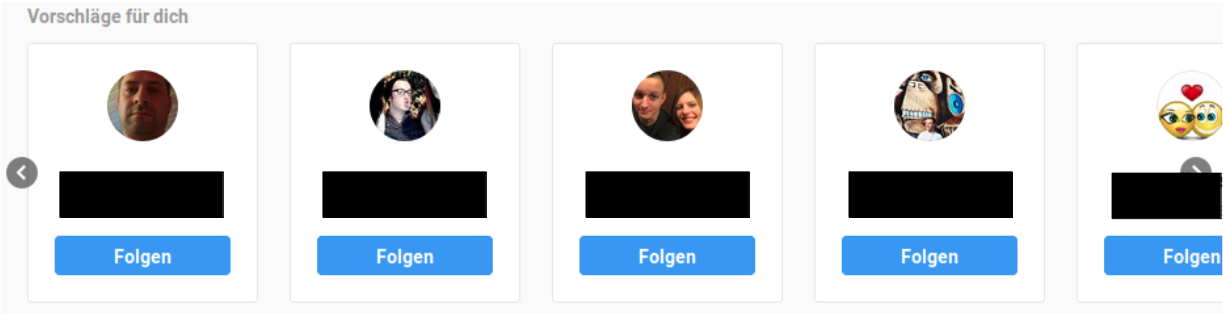
\includegraphics[ scale=0.35]{bilder/instagram_vorschlaege.png}
			\caption{Container mit Profil-Vorschlägen}
			\label{img:instagram_vorschlaege}
		\end{figure}
		
		Falls es sich um ein öffentlich frei zugängliches Profil handelt, kann eine Liste der abonnierten Kontakte angezeigt werden. Hierbei handelt es sich um ein scrollbares Pop-Up-Fenster \ref{img:instagram_abonniert}. Vergleichbar zur Methode bei einer privaten Profilseite, wird hier ebenfalls Schritt-für-Schritt durchgescrollt. Dadurch wird jedes einzelne Profil geladen und der dazugehörig Link, zur dieser Profilseite, kann dadurch ausgelesen werden. 
		
		
		
		\begin{figure}[H]
			\centering
			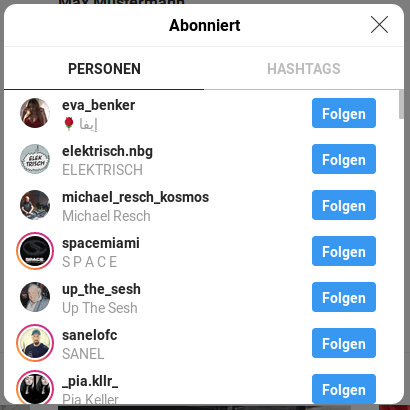
\includegraphics[ scale=0.35]{bilder/instagram_abonniert.png}
			\caption{Pop-up-Fenster mit abonnierten Profilen}
			\label{img:instagram_abonniert}
		\end{figure}
	
		Die Herausforderung besteht darin, dass nicht zu schnell gescrollt werden darf. Aus diesem Grund wird ein Algorithmus \ref{lst:AlgoZumDurchscrollen} verwendet, welcher einem menschlichen Verhalten ähneln soll. Hierbei wird zuallererst das Pop-up-Fenster gesucht und festgelegt. Anschließend wir die Anzahl der abonnierten Profile gezählt. Die Anzahl der Profile wird dazu verwendet, dass der Algroithmus weiß wie weit nach unten geblättert werden muss, um alle Profil zu laden.\\
		Im ersten Schritt, wird das Fenster nur ein sechstel des möglichen Bereichs nach unten gescrollt. Dadurch werden weitere Profile geladen. Wenn direkt nach ganz unten geblättert wird, wäre dies beim ersten Scrollvorgang zu schnell. In diesem Fall werden keine Kontakte geladen. Es werden lediglich Profil von sehr bekannten Instagram-Usern angezeigt, die von dieser Person abonniert wurden.\\
		In den nächsten Schritte wird das Fenster jeweils ganz nach unten verschoben. Dadurch werden alle Profile geladen. Sobald alle Links bekannt sind, wird eine URL zu den entsprechenden Profilseiten erstellt. Diese Seiten werden anschließen wie jede andere Seite ausgelesen und nach Information durchsucht. Infolgedessen wird die gewonnene Information jedes Profils mit der Information der Zielperson verglichen. Die Suche wird bei einem beliebigen Treffer beendet. Anschließend wird die gefunden Information mit dem Namen des Benutzers der Profilseite gespeichert. Diese abgespeicherten Daten können später zur E-Mail-Generierung verwendet werden.\\
		
		\begin{lstlisting}[caption=Herunterscrollen des Pop-up Fensters,label={lst:AlgoZumDurchscrollen}]
			# Find the pop-up window
			pop_up = self.browser.find_element_by_xpath('/html/body/div[2]
					/div/div[2]')        
			# find number of followers
			all_following = int(self.browser.find_element_by_xpath("//li[2]
					/a/span").text)
			# scroll down the page
			for i in range(int(all_following / 6)):
				if i == 0:
					self.browser.execute_script("arguments[0].scrollTop = 
							arguments[0].scrollHeight/5", pop_up)
					time.sleep(2)
				else:
					self.browser.execute_script("arguments[0].scrollTop = 
							arguments[0].scrollHeight", pop_up)
				time.sleep(random.randint(500, 1000) / 1000)
		\end{lstlisting}



\section{Speicherung der gewonnenen Daten}
Die gespeicherten Daten werden von verschiedenen Klassen benötigt. Aus diesem Grund muss es möglich sein, dass andere Klassen auf die Speicherstruktur zugreifen können. Des Weiteren wird eine gute Struktur vorausgesetzt, damit auf einzelne Attribute der Person zugegriffen werden kann. Es ist nicht notwendig, dass die Daten nach Programmende abrufbar sind. Infolgedessen wird keine externe Speicherung in einer Datenbank oder in einer Datei vorausgesetzt.\\
Eine mögliche Speicherung der Daten wäre in einer SQL-Datenbank. Alternativ könnten die Personendaten in einer externen Datei oder mit Hilfe einem Personenobjekt gespeichert werden.\\
Eine SQL-Datenbank bringt eine gute Speicherstruktur mit sich. Allerdings sind mit einer SQL-Datenbank aufwendigere Speicher-und Abrufvorgänge verbunden. Die externe Speicherung in einer Datei wie CVS oder TXT ist keine Anforderung. Auf eine SQL-Datenbank sowie auf eine externe Datei, lässt sich mit jeder Klasse darauf zugegriffen. Dennoch wird ein Personenobjekt verwendet. Dadurch werden keine unnötigen Speicher- und Lesezugriffe benötigt. Darüber hinaus lässt sich das Personenobjekt an die entsprechenden Klassen übergeben.
	\subsection{Implementierung der Personenklasse}
	Die gewonnenen Daten werden in einem Personenobjekt, wie in Listing \ref{lst:AlgoPersonobject} dargestellt, gespeichert. Dabei werden die vom Anwender eingegebenen Daten direkt in das Personenobjekt übertragen. Die gewonnen Informationen werden in Form einer Liste hinzugefügt. Falls bei der Kontaktanalyse ein Treffer gemacht wurde, kann diese Information in dem Attribute "'contacts\_information gespeichert werden. Hierbei wird zuerst der vollständige Kontaktname und anschließend die übereinstimmende Information gespeichert. Ein Beispiel hierfür wäre ["'Max Mustermann"',"'Fußball"']\\
	
	\begin{lstlisting}[caption=Personklasse,label={lst:AlgoPersonobject}]
	class Person(object):
		def __init__(self):
			self.first_name = input("Vorname: ")
			self.second_name = input("Nachname: ")
			self.place_of_residence = input("Wohnort: ")
			self.year_of_birth = input("Geburtsjahr: ")
			self.institution = input("Institution: ")
			self.instagram_name = input("Instagram Benutzername: ")
			self.facebook_name = input("Facebook Benutzername: ")
			self.twitter_name = input("Twitter Benutzername: ")
			self.input_email = input("E-Mail-Adresse: ")
			self.occupation = []
			self.hobbies = []
			self.universities = []
			self.founded_mails = []
			self.locations = []
			self.contacts_information = []
	\end{lstlisting}
	
			% Masterdatei einen sinnvollen
		% Kommentar erhalten
%%Kapitel der Umsetzung

\chapter{Informationsbeschaffung einer großen Anzahl von Person}  %Name des Kapitels
\label{cha:Informationsbeschaffung einer grossen Anzahl von Person} %Label des Kapitels
\section{Festlegung einer ausgewählten Webseite}
Warum Fupa?
\section{Aufbau einer Webseite analysieren}

\section{Erstellung eines internen Web Crawlers} %Unterunterkapitel
	\label{sse:}
	Damit die Webseite \textit{www.fupa.net} komplett nach Spielerdaten durchsucht werden kann, wird ein interner Web Crawler benötigt. Dieser wird sich anhand den internen Links, über die ganze Seite hinweg, durchhangeln.\\
	Für die Erstellung eines hartkodierten Web Crawlers muss zuerst einmal der komplette Aufbau einer Webseite bekannt sein. Dies lässt sich einfach mit Hilfe der Entwicklertools in einem Browser durchführen. %TODO Möglicherweise Bild von dem Aufbau der Seite
	
	\subsection{Funktionsweise des Web Crawlers}
	Links mit Spielerinformationen speichern.
	Die Funktionsweise des Web Crawlers besteht darin, dass das Programm auf der Startseite von Fupa.net beginnt nach links zu suchen und diesen folgt.
	\subsection{Probleme bei der Erstellung} %Unterkapitel 3. Ordnung
	\begin{enumerate}
		\item Python hat einen verkürzten und erkennbaren Standard http-Header. Dieser wird von vielen Administratoren geblockt und mit der Fehlermeldung 451 erkennbar gemacht. 451 for legal reason
		\item Honeypots gewollt oder ungewollt, hier Kalender darstellung mit links zu neuen Jahren die eine sehr hohe bis überhaupt keine Begrenzung haben.
		\item Rekursion erreicht schnell die Maximale tiefe von 1500.
		\item Zu langsamer Algorithmus
	\end{enumerate}
	
	
	\subsection{Lösungen}
	\begin{enumerate}
		\item http-Header selber konfigurieren
		\item Links mit möglichen Honeypots nicht beachten
		\item Stack Klasse schreiben damit keine Rekursion benötigt wird
		\item Algorithmus anpassen auf fupa-Webseite
	\end{enumerate}

\section{Auslesen der Webseite durch Hartkodierung}

\section{Datenverwaltung und Speicherung}
%TODO Speicherung kommt in Umsetzung, da es nicht zur Kernfrage gehört.
Für die Speicherung der gewonnen Daten kann eine SQL-Datenbank erstellt werden.
Als Alternative kann eine Datei angelegt werden, bei der alle Daten zu allen Personen gut strukturiert gespeichert werden können. Eine Möglichkeit dafür wäre das Dateiformat \textit{CSV} oder \textit{TXT}.		% z.B. den Titel des Kapitels
%Kapitel der Umsetzung

\chapter{Generierung der Phishing-E-Mail}  %Name des Kapitels
\label{cha:ErstellungeinerPhishing-Mail} %Label des Kapitels
In diesem Kapitel wird die Umsetzung zur Erstellung einer Phishing-Mail beschrieben. Dabei wir zuerst auf die Implementierung des Algorithmus zur Adressgenerierung eingegangen. Anschließend werden die E-Mail-Muster vorgestellt. Im letzten Abschnitt wird die Umsetzung zum Versenden einer Phishing-E-Mail aufgezeigt. 

\section{Implementierung der Methode zur Generierung der E-Mail-Adressen}	
Für den zu entwickelnden Algorithmus wird eine eigene Klasse erstellt. Diese Klasse ist ausschließlich für die Generierung der E-Mail-Adressen zuständig. Diese Methode zeigt, wie aus personenbezogenen Daten eine mögliche E-Mail-Adresse generiert werden kann. Jedoch wird in der Anwendung keine Phishing-Mail an eine dieser Adressen, welche mit der Methode erzeugt wurden, versendet. Es dient ausschließlich als Beweis für die Durchführbarkeit dieser Methode.

	\subsection{Funktion des eigenen Algorithmus}
	Der lokale Teil einer E-Mail-Adresse befindet sich vor dem At-Zeichen. Dieser kann aus verschiedensten Daten bestehen. Allerdings wird in den meisten Fällen der bürgerlichen Namen verwendet. \cite{NameAlsEMail} Aus diesem Grund verwendet der Algorithmus die Personenattribute Vorname, Nachname und zusätzlich das Geburtsjahr.\\
	Im ersten Schritt wird kontrolliert, welche Daten bekannt sind. Im Idealfall sind das alle drei Attribute. Im zweiten Schritt wird festgelegt, aus welchen Daten der lokale Teil bestehen kann. Im Folgenden sind möglichen Kombinationen aufgezeigt.
	
	\textit{Vorname;}\\
	\textit{Nachname;}\\
	\textit{Vorname, Nachname;}\\
	\textit{Vorname, Nachname, vollständiges Geburtsjahr;}\\
	\textit{Vorname, Nachname, Kurzform des Geburtsjahrs;}
	
	Ein lokaler Teil kann somit aus mehreren Daten bestehen. Es kann vorkommen, dass anstatt "'Max Mustermann"' "'Mustermann Max"' als lokaler Namen verwendet wird. Aus diesem Grund wird für jeden lokalen Teil, der aus mehreren Daten besteht, eine Permutation ohne Wiederholung angewendet. Dadurch werden alle möglichen Kombinationen von Anordnungen der bekannten Daten generiert. Dabei wird zusätzlich auf die Reihenfolge der Anordnungen geachtet. Somit ist das Element "'Max Mustermann"' und "'Mustermann Max"' eine eigene Kombination. Es werden zusätzlich die selben Kombinationen mit den Trennzeichen "'."', "'\_"' und "'-"' erstellt und in einer Liste gespeichert. Das Ergebnis einer Permutation über die Attribute "'Vorname"' und "'Nachname"' werden nachstehen dargestellt.
	
	\textit{[Vorname], [Nachname], [Vorname \& Nachname], Vorname \& '.'\& Nachname], [Vorname \& '\_' \& Nachname], [Vorname \& '-' \& Nachname], [Nachname \& Vorname], [Nachname \& '.' \& Vorname], [Nachname \& '\_' \& Vorname], [Nachname \& '-' \& Vorname]}
	
	Für den Domainteil werden die bekannte Mailprovider in Deutschland verwendet. Dazu gehören die Provider GMX, WEB.DE, Gmail, T-Online, Freenet und 1\&1.\cite{AnbieterMail}. Das bedeutet, es wird für jeden lokalen Namen eine E-Mail-Adresse mit den jeweiligen Mailprovidern und der Landeskennung "'de"' erzeugt. Die folgende Tabelle  zeigt die erzeugten E-Mail-Adressen des Algorithmus für die Daten "'Marco"', "'Lang"' und "'1995"'. Es sind nur die Mailadressen für die Provider WEB.DE, Gmail und Freenet aufgelistet.
	
	\begin{center}
		%\begin{table}[h!]
		\scriptsize
		\begin{longtable}{c|c|c}
			\label{EMailAdressen}

			%\centering
			%\scriptsize
			%\begin{tabular}{c|c|c}
				marco@web.de& marco@gmail.com& marco@freenet.de\\ 
				lang@web.de& lang@gmail.com& lang@freenet.de\\
				marcolang@web.de& marcolang@gmail.com& marcolang@freenet.de\\
				marco.lang@web.de& marco.lang@gmail.com& marco.lang@freenet.de\\ 
				marco\_lang@web.de& marco\_lang@gmail.com& marco\_lang@freenet.de\\ 
				marco-lang@web.de& marco-lang@gmail.com& marco-lang@freenet.de\\
				langmarco@web.de& langmarco@gmail.com& langmarco@freenet.de\\
				lang.marco@web.de& lang.marco@gmail.com& lang.marco@freenet.de\\
				lang\_marco@web.de& lang\_marco@gmail.com& lang\_marco@freenet.de\\
				lang-marco@web.de& lang-marco@gmail.com& lang-marco@freenet.de\\
				marcolang1995@web.de& marcolang1995@gmail.com& marcolang1995@freenet.de\\
				marco.lang.1995@web.de& marco.lang.1995@gmail.com& marco.lang.1995@freenet.de\\
				marco\_lang\_1995@web.de& marco\_lang\_1995@gmail.com& marco\_lang\_1995@freenet.de\\
				marco-lang-1995@web.de& marco-lang-1995@gmail.com& marco-lang-1995@freenet.de\\ 
				marco1995lang@web.de& marco1995lang@gmail.com& marco1995lang@freenet.de\\
				marco.1995.lang@web.de& marco.1995.lang@gmail.com& marco.1995.lang@freenet.de\\ 
				marco\_1995\_lang@web.de& marco\_1995\_lang@gmail.com& marco\_1995\_lang@freenet.de\\
				marco-1995-lang@web.de& marco-1995-lang@gmail.com& marco-1995-lang@freenet.de\\
				langmarco1995@web.de& langmarco1995@gmail.com& langmarco1995@freenet.de\\
				lang.marco.1995@web.de& lang.marco.1995@gmail.com& lang.marco.1995@freenet.de\\ 
				lang\_marco\_1995@web.de& lang\_marco\_1995@gmail.com& lang\_marco\_1995@freenet.de\\
				lang-marco-1995@web.de& lang-marco-1995@gmail.com& lang-marco-1995@freenet.de\\
				lang1995marco@web.de& lang1995marco@gmail.com& lang1995marco@freenet.de\\
				lang.1995.marco@web.de& lang.1995.marco@gmail.com& lang.1995.marco@freenet.de\\ 
				lang\_1995\_marco@web.de& lang\_1995\_marco@gmail.com& lang\_1995\_marco@freenet.de\\ 
				lang-1995-marco@web.de& lang-1995-marco@gmail.com& lang-1995-marco@freenet.de\\ 
				1995marcolang@web.de& 1995marcolang@gmail.com& 1995marcolang@freenet.de\\
				1995.marco.lang@web.de& 1995.marco.lang@gmail.com& 1995.marco.lang@freenet.de\\ 
				1995\_marco\_lang@web.de& 1995\_marco\_lang@gmail.com& 1995\_marco\_lang@freenet.de\\ 
				1995-marco-lang@web.de& 1995-marco-lang@gmail.com& 1995-marco-lang@freenet.de\\
				1995langmarco@web.de& 1995langmarco@gmail.com& 1995langmarco@freenet.de\\
				1995.lang.marco@web.de& 1995.lang.marco@gmail.com& 1995.lang.marco@freenet.de\\ 
				1995\_lang\_marco@web.de& 1995\_lang\_marco@gmail.com& 1995\_lang\_marco@freenet.de\\
				1995-lang-marco@web.de& 1995-lang-marco@gmail.com& 1995-lang-marco@freenet.de\\
				marcolang95@web.de& marcolang95@gmail.com& marcolang95@freenet.de\\
				marco.lang.95@web.de& marco.lang.95@gmail.com& marco.lang.95@freenet.de\\ 
				marco\_lang\_95@web.de& marco\_lang\_95@gmail.com& marco\_lang\_95@freenet.de\\ 
				marco-lang-95@web.de& marco-lang-95@gmail.com& marco-lang-95@freenet.de\\ 
				marco95lang@web.de& marco95lang@gmail.com& marco95lang@freenet.de\\ 
				marco.95.lang@web.de& marco.95.lang@gmail.com& marco.95.lang@freenet.de\\ 
				marco\_95\_lang@web.de& marco\_95\_lang@gmail.com& marco\_95\_lang@freenet.de\\
				marco-95-lang@web.de& marco-95-lang@gmail.com& marco-95-lang@freenet.de\\
				langmarco95@web.de& langmarco95@gmail.com& langmarco95@freenet.de\\ 
				lang.marco.95@web.de& lang.marco.95@gmail.com& lang.marco.95@freenet.de\\ 
				lang\_marco\_95@web.de& lang\_marco\_95@gmail.com& lang\_marco\_95@freenet.de\\ 
				lang-marco-95@web.de& lang-marco-95@gmail.com& lang-marco-95@freenet.de\\
				lang95marco@web.de& lang95marco@gmail.com& lang95marco@freenet.de\\
				lang.95.marco@web.de& lang.95.marco@gmail.com& lang.95.marco@freenet.de\\ 
				lang\_95\_marco@web.de& lang\_95\_marco@gmail.com& lang\_95\_marco@freenet.de\\ 
				lang-95-marco@web.de& lang-95-marco@gmail.com& lang-95-marco@freenet.de\\
				95marcolang@web.de& 95marcolang@gmail.com& 95marcolang@freenet.de\\ 
				95.marco.lang@web.de& 95.marco.lang@gmail.com& 95.marco.lang@freenet.de\\ 
				95\_marco\_lang@web.de& 95\_marco\_lang@gmail.com& 95\_marco\_lang@freenet.de\\
				95-marco-lang@web.de& 95-marco-lang@gmail.com& 95-marco-lang@freenet.de\\
				95langmarco@web.de& 95langmarco@gmail.com& 95langmarco@freenet.de\\
				95.lang.marco@web.de& 95.lang.marco@gmail.com& 95.lang.marco@freenet.de\\ 
				95\_lang\_marco@web.de& 95\_lang\_marco@gmail.com& 95\_lang\_marco@freenet.de\\ 
				95-lang-marco@web.de& 95-lang-marco@gmail.com& 95-lang-marco@freenet.de
		%	\end{tabular}
		
		%\end{table}
	\end{longtable}
	\end{center}
	

\section{Implementierung der E-Mail-Muster}
Ein E-Mail-Muster entspricht einem Lückentext, bei dem die entsprechenden Lücken mit den gewonnen Daten ergänzt werden. Die Texte müssen so erstellt werden, dass sie die Zielperson ansprechen. Aus diesem Grund muss für jede Kombination der gewonnenen Daten ein Muster zur Verfügung stehen. Zusätzlich stellt sich die Frage, wie die E-Mail-Texte möglichst passend kategorisiert werden können.

	\subsection{Kategorien erstellen}
	Die Muster können in zwei große Kategorien unterteilt werden. Es gibt eine private und eine berufliche Kategorie. Der Unterschied zwischen privat und beruflich besteht in der Art und Weise wie ein Text geschrieben wird. Genaugenommen bedeutet das, dass ein privates Muster in einer Umgangssprache und ein berufliches in einer formelleren Sprache erstellt wird. Diese beiden Kategorien haben weitere Unterkategorien, welche verschiedene Kombinationen aus den personenbezogenen Daten verwenden.\\
	Um die Kategorie zu erkennen, werden zu Beginn Abfragen gestartet. Dadurch wird kontrolliert, welche Daten bekannt sind. Im Fall, dass die Institution oder die Tätigkeit der Zielperson bekannt ist, wird ein berufliches Muster gewählt. Andernfalls wird ein privates Muster verwendet.
	
		\subsubsection{Berufliche E-Mail-Muster}
		\label{subsubsec:beruflicheMuster}
		Die beruflichen E-Mail-Muster sind in den folgenden Bildern aufgezeigt. Die Reihenfolge zur Auswahl der Muster im laufenden Programm entspricht der Reihenfolge der Bilder. Dabei werden die kursiv geschriebenen Wörter in den Bildern mit den gewonnenen Daten über die Zielperson ersetzt.\\ 
		Das Bild \ref{img:NameInstitution} beschreibt ein berufliches Muster, welches die Personenattribute Nachname und Institution verwendet. Im Bild \ref{img:NachnameTätigkeit1} ist ein Muster mit den Attributen Nachname und Tätigkeit aufgezeigt. Das Bild \ref{img:NachnameTätigkeit} zeigt das Muster mit denselben Attributen, wobei die Tätigkeit zu Beginn abgefragt wurde. Infolgedessen kann dieses Datenelement als Entscheidungskriterium für die Auswahl eines Musters verwendet werden. In diesem bestimmten Fall wurde das Muster mit dem festgesetzten Wort "'Professor"' gewählt. Im letzten Bild wird das berufliche Muster für die Daten Nachname, Tätigkeit und Institution beschrieben.
			\begin{figure}[h!]
				\label{img:NameInstitution}
				\fbox{\parbox{\linewidth}{\texttt{SUBJECT:\quad \textit{Musterinstitution} - Netzwerkänderungen\\\\
							Hallo \textit{Herr Mustermann},\\
							wir bauen unsere Netzwerkstruktur um. Bitte registrieren Sie sich unter der folgenden Webseite, damit wir Sie in das neue System aufnehmen können.\\https://badlink.com\\\\Mit freundlichen Grüßen\\\\Ihr IT-Team der \textit{Musterinstitution}}}}
				\caption{Ein berufliches E-Mail-Muster mit den Personenattributen Nachname und Institution }
			\end{figure}
		
			\begin{figure}[h!]
				\label{img:NachnameTätigkeit1}
				\fbox{\parbox{\linewidth}{\texttt{SUBJECT:\quad \textit{Mustertätigkeit} gesucht - Im Auftrag des BRD\\\\
							Hallo \textit{Herr Mustermann},\\die Bundesrepublik Deutschland sucht einen kompetenten \textit{Mustertätigkeit}.
							Haben Sie Interesse an einer neuen Herausforderung unter optimalen Arbeitsbedingungen?\\
							Im Anhang finden Sie die offizielle Stellenausschreibung mit den dazugehörigen Voraussetzungen und Gehaltsstufen.\\
							\\\\\
							Ihr Karriere-Team der Bundesrepublik Deutschland}}}
				\caption{Ein berufliches E-Mail-Muster mit den Personenattributen Nachname und Tätigkeit}
			\end{figure}
		
			\begin{figure}[h!]
				\label{img:NachnameTätigkeit}
				\fbox{\parbox{\linewidth}{\texttt{SUBJECT:\quad Feedback zur Ausarbeitung\\\\
							Hallo \textit{Herr} Professor \textit{Mustermann},\\
							wie besprochen befindet sich im Anhang meine vorläufige Ausarbeitung. Könnten Sie diese bitte erneut überprüfen und mir ein Feedback geben?\\\\Mit freundlichen Grüßen\\\\	Max Mustermann}}}
				\caption{Ein berufliches E-Mail-Muster mit dem Personenattribut Nachname und einer festgesetzten Tätigkeit}
			\end{figure}
		
			\begin{figure}[h!]
				\label{img:NachnameTätigkeitInsitution}
				\fbox{\parbox{\linewidth}{\texttt{SUBJECT:\quad \textit{Mustertätigkeit} bei der \textit{Musterinstitution}\\\\
							Hallo \textit{Herr Mustermann},\\
							als \textit{Mustertätigkeit} bei der \textit{Musterinstitution}, stehen Ihnen nun alle Möglichkeiten offen. Sehen Sie nun Ihre neuen Möglichkeiten unter folgendem Link an.\\
							https://badlink.com\\\\Mit freundlichen Grüßen\\\\Ihr Team der \textit{Musterinstitution}}}}
				\caption{Ein berufliches E-Mail-Muster mit den Personenattributen Nachname, Tätigkeit und Institution }
			\end{figure}
			
		\subsubsection{Private E-Mail-Muster}
			Im Nachfolgenden werden die privaten E-Mail-Muster aufgezeigt. Die Ersetzung der kursiven Wörter sowie die Reihenfolge der Muster-Auswahl ist identisch zum vorherigen Kapitel \ref{subsubsec:beruflicheMuster}.\\
			Im ersten Bild wird ein privates E-Mail-Muster beschrieben, welche die gewonnenen Kontaktinformationen verwendet. Genaugenommen ist das der Kontaktname und die Kontaktinformation. Diese Kontaktinformation ist identisch zu einer Information über die Zielperson. Das nächste Bild beschreibt ein Muster, bei dem die Personendaten Vorname und Hobby verwendet werden. Das Bild \ref{img:VornameJahrgang} zeigt die Verwendung des Vornamens und des Geburtsjahrs in einem E-Mail-Muster. Das letzte Muster verwendet die Personenattribute Vorname und Ort. Hierfür wird  der gefundene Ort verwendet.\\
			\FloatBarrier
			
			\begin{figure}[h!]
				\fbox{\parbox{\linewidth}{\texttt{SUBJECT:\quad Fragen bzgl. \textit{Kontaktinformation}\\\\Hi \textit{Max},\\ hier ist \textit{Kontaktname}. Bezüglich \textit{Kontaktinformation} hätte ich noch ein paar Fragen an dich...\\ Könntest du vielleicht in den Anhang schauen und bewerten, was ich dazu so rausgesucht habe?\\Vielen Danke im Voraus!\\\\\textit{Kontaktname}}}}
			\caption{Ein privates E-Mail-Muster mit den Personenattributen Vorname, Kontaktname und Kontaktinformation}
			\end{figure}
			\FloatBarrier
			\begin{figure}[h!]
				\fbox{\parbox{\linewidth}{\texttt{SUBJECT:\quad Verbessere deine Technik im \textit{Musterhobby}\\\\
							Hi \textit{Max},\\ damit du deine Leistung im \textit{Musterhobby} verbessern kannst, musst du unbedingt die Techniken deiner Vorbilder anschauen!\\Im Anhang befindet sich darüber eine kleine Übersicht.\\\\Dein Team der deutschen Förderung}}}
				\caption{Ein privates E-Mail-Muster mit den Personenattributen Vorname und Hobby}
			\end{figure}
		
			\begin{figure}[h!]
				\label{img:VornameJahrgang}
				\fbox{\parbox{\linewidth}{\texttt{SUBJECT:\quad Jahrgang \textit{Geburtsjahr}\\\\
							Hi \textit{Max},\\dieses Jahr findet ein Treffen für alle Personen, die \textit{Geburtsjahr} geboren sind, statt.\\Im Anhang befindet sich eine Liste mit den Leuten die bereits zugesagt haben.\\\\Dein Orga-Team}}}
				\caption{Ein privates E-Mail-Muster mit den Personenattributen Vorname und Jahrgang}
			\end{figure}
		
			\begin{figure}[h!]
				\fbox{\parbox{\linewidth}{\texttt{SUBJECT:\quad Streetfood-Festival in \textit{Musterort}\\\\
							Hi \textit{Max},\\dieses Jahr findet das erste STREETFOOD-FESTIVAL in \textit{Musterort} statt. Im Anhang befindet sich der Plan, auf dem alles weitere erklärt wird.\\
							Wir freuen uns auf dich!\\\\Dein Streefood-Team aus \textit{Musterort}}}}
				\caption{Ein privates E-Mail-Muster mit den Personenattributen Vorname und Ort}
			\end{figure}
		
		\FloatBarrier
\section{Versenden einer Phishing-E-Mail}
Damit eine Phishing-Mail beispielhaft versendet werden kann, wird eine Absender-Adresse benötigt. Sehr große Provider wie Gmail oder Yahoo sind dafür nicht optimal. Das hat den Grund, dass viele Spammer diese Provider in der Vergangenheit verwendet haben. Dadurch werden diese Adressen gerne öfter überprüft. Kleine Provider wie GMX sind dagegen nicht so bekannt. Ein weiterer Vorteil von GMX ist, dass ein Account ohne eine weitere gültige E-Mail-Adresse erzeugt werden kann. Das spricht für GMX, da bei einem gefälschten Account keine Verbindung zu einem verwendeten Profil besteht. Des Weiteren ist dieser kleine Provider großen Plattformen wie Facebook fremd und wird dadurch weniger streng überprüft. Aus den erwähnten Gründen wird eine E-Mail-Adresse bei GMX erstellt.\cite{Bazzell}\\
Mithilfe der erzeugten Adresse und einem Python Skript kann eine Phishing-Mail beispielhaft versendet werden. Dazu wird die Python Bibliothek "'smtplib"' verwendet. Im ersten Schritt werden die erstellten E-Mail-Daten wie Sender-Adresse, Ziel-Adresse, Betreff und Inhalt einer mehrteiligen Nachricht hinzugefügt. Als nächstes wird die Verbindung mit dem GMX-Mailserver aufgebaut. Nach einer erfolgreichen Anmeldung kann eine E-Mail versendet werden. 










			% um für Korrekturen oder Umstellungen

%Kapitel des Evaluation

\chapter{Evaluation der Implementation}  %Name des Kapitels
\label{cha:Evaluation der Implementation} %Label des Kapitels
\section{Validierung des Gesamtkonzeptes}
Das Gesamtkonzept dieser Anwendung wurde entsprechend den Anforderungen umgesetzt. Eine große Herausforderung ist die Identifizierung einer Person. Dazu wurde die Methode zur Generierung von Identifikationsschlüsseln erstellt. Darüber hinaus wurden die Sucher-URLs optimiert, damit die Suchergebnisse reduziert und verbessert werden. Dennoch besteht die Möglichkeit der Verwechslung einer Person, wenn sich die gefundene Profile sehr ähneln.\\
Zum Herausfiltern von wichtigen Informationen wurden Schlüsselwörter aus dem Text erzeugt und mit den Elementen aus den Wortsammlungen verglichen. Dabei bestehen alle Elemente, außer die der Wortsammlung Institution, aus einem Wort. Das bedeutet, es können nur Schlüsselwörter bestehend aus einem Wort gefunden werden. Dagegen kann eine Institution mehrere Wörter enthalten. Allerdings kann in diesem Fall die Häufigkeit des Vorkommens einer Institution auf einer Webseite nicht erkannt werden. Somit besteht bei beiden Fällen die Gefahr von Fehlinterpretation oder Missachtung einer Information.\\
Für die Bestimmung, welche Daten verwendet werden, wurde ein Algorithmus entwickelt. Dieser berechnet unter Beachtung von bestimmten Kriterien einen Score. Anschließend wird das Element mit der höchsten Score ausgewählt. Diese Berechnung kann im Fall, dass nur ein Element einer Kategorie auf einer Webseite gefunden wurde, zu Problemen führen. Bei dieser Ausnahme wird das eine Element sehr hoch gewichtet. Dadurch kann es zu einer fehlerhaften Auswahl kommen. Jedoch ist die Berechnung der Wertung unter Berücksichtigung der Kriterien nötig, um einen dauerhaften Auswahlfehler zu vermeiden.\\
Die Phishing-E-Mails werden mit Mustern erzeugt. Dadurch enthält die E-Mail einen sinnvollen Inhalt mit einer korrekten Grammatik. In einzelnen Fällen kann es jedoch zu sonderbaren Formulierungen kommen.

\section{Beschreibung und Motivation der Testfälle}
Bei den Testfällen wurden verschiedene Personen mit unterschiedlichen Daten gesucht. Für jede Zielperson wurde eine Einverständniserklärung eingeholt. Somit besteht jeder einzelne Testfall aus einer Suche nach einer realen Personen.
	\subsection{Testfall 1}
	\label{subsec:Testfall1}
	Im ersten Testfall wurde nach der Person mit dem Namen "'Marco Lang"' und dem Wohnort Tettnang gesucht. Dabei ist zusätzlich der Instagram-Benutzername dieser Zielperson bekannt.
	\subsubsection{Ergebnisse}
		\begin{figure}[h!]
			\fbox{\parbox{\linewidth}{\texttt{Vorname: marco\\
						Nachname: lang\\
						Wohnort/Standort: tettnang\\
						Geburtsjahr: 1995\\
						Ort: tettnang\\
						Tätigkeit: None\\
						Hobby: fitness\\
						Institution: None\\
						E-Mails:  []\\
						Kontaktinformation:  ['sophie', 'fitness']\\\\
						Phishing-Mail:\\
						Betreff: Fragen bzgl. Fitness\\
						Hi Marco,\\
						hier ist Sophie. Bezüglich Fitness hätte ich noch ein paar fragen an dich...\\
						Könntest du zufällig in den Anhang schauen und bewerten was ich da so rausgesucht habe?\\\\
						Grüße,\\					
						Sophie}}}
			\caption{Programmausgabe zu dem Testfall 1}
		\end{figure}
		\FloatBarrier
	\subsection{Testfall 2}
	\label{subsec:Testfall2}
	Für diesen Testfall wird nach der Person "'Anika Zeilmann"' gesucht. Der Wohnort ist bei dieser Suche keine Stadt, sondern die Gemeinde Heidesheim aus dem Bundesland Rheinland-Pfalz. Es werden keine zusätzlichen Personendaten angegeben.
		\subsubsection{Ergebnisse}
			\begin{figure}[h!]
			\fbox{\parbox{\linewidth}{\texttt{Vorname: anika\\
						Nachname: zeilmann\\
						Wohnort: heidesheim\\
						Geburtsjahr: None\\
						Ort: heidesheim\\
						Tätigkeit: student\\
						Hobby: basketball\\
						Institution: hochschule mainz\\
						E-Mails: []\\
						Kontaktinformation: []\\\\
						Phishing-Mail:\\
						Betreff: Rückmeldung - Hochschule Mainz\\
						Hallo Frau Zeilmann,\\
						leider ist und ein Fehler unterlaufen. Aus diesem Grund müssen sie sich erneut zurückmelden.
						Um den Vorgang zu beschleunigen, klicken Sie bitte auf den folgenden Link.\\
						https://badlink.com\\\\
						Mit freundlichen Grüßen\\\\
						Ihr Team der Hochschule Mainz}}}
			\caption{Programmausgabe zu der Suche "'Anika Zeilmann"' \& "'Heidesheim"'}
		\end{figure}
		\FloatBarrier
	\subsection{Testfall 3}
	\label{subsec:Testfall3}
	Für diesen Testfall ist die Zielperson "'Wolfgang Lang"'. Hierbei wird zweimal nach der gleichen Person gesucht. Allerdings mit zwei unterschiedlichen Orten. Der erste Ort ist Meckenbeuren und entspricht dem Arbeitsort. Im zweiten Fall wird der Wohnort Tettnang verwendet.
		\subsubsection{Ergebnisse}
			\begin{figure}[h!]
				\fbox{\parbox{\linewidth}{\texttt{Vorname: wolfgang\\
				Nachname: lang\\
				Wohnort: meckenbeuren\\
				Geburtsjahr: None\\
				Ort: meckenbeuren\\
				Tätigkeit: prokurist\\
				Hobby: politik\\
				Institution: p+w metallbau gmbh \& co. kg\\
				E-Mails: [lang@pw-metallbau.de]\\
				Kontaktinformation: []\\\\
				Phishing-Mail:\\
				Betreff: Prokurist bei der P+W Metallbau GmbH \& Co. KG\\
				Hallo Herr Lang,\\
				als Prokurist bei der Institution P+W Metallbau GmbH \& Co. KG, stehen Ihnen nun alle Möglichkeiten offen. Sehen Sie sich die neuen Möglichkeiten unter folgendem Link an.\\
				https://badlink.com\\\\
				Mit freundlichen Grüßen\\\\
				Ihr Karriere-Team der Institution P+W Metallbau GmbH \& Co. KG}}}
				\caption{Programmausgabe zum Tesfall 1 - Meckenbeuren}
			\end{figure}
			\FloatBarrier
			\begin{figure}[h!]
				\fbox{\parbox{\linewidth}{\texttt{Vorname: wolfgang\\
							Nachname: lang\\
							Wohnort: tettnang\\
							Geburtsjahr: None\\
							Ort: meckenbeuren\\
							Tätigkeit: bäcker\\
							Hobby: reisen\\
							Institution: europäische fachhochschule\\
							E-Mails: []\\
							Kontaktinformation: []\\\\
							Phishing-Mail:\\
							Betreff: Bäcker bei der Institution Europäische Fachhochschule\\
							Hallo Herr Lang,\\
							als Bäcker bei der Institution Europäische Fachhochschule, stehen Ihnen nun alle Möglichkeiten offen. Sehen Sie sich die neuen Möglichkeiten unter folgendem Link an.\\
							https://badlink.com\\\\
							Mit freundlichen Grüßen\\\\
							Ihr Karriere-Team der Institution Europäische Fachhochschule}}}
				\caption{Programmausgabe zum Tesfall 1 - Tettnang}
			\end{figure}
			\FloatBarrier
			
\section{Übersicht und Bewertung der erzielten Ergebnisse}
	\subsection{Bewertung Testfall 1}
	Im Testfall \ref{subsec:Testfall1} wurde mit Hilfe eines vollständigen Namens, dem Wohnort und dem einmaligen Instagram-Benutzername gesucht. Dabei wurde ein richtiges Personenprofil erstellt.\\
	Das Geburtsjahr, der Ort, das Hobby und die Kontaktinformation ist gefunden worden und spricht mit dem tatsächlichen Personenprofil überein. Das Hobby "'Fitness"' wird auf dem Instagram-Profil der Ziel- sowie der Kontaktperson gefunden. Allerdings hat der Kontakt keinen vollständigen Namen angegeben. Dadurch konnte nur der Vorname "'Sophie"' gefunden werden.\\
	Die Anrede für die Phishing-Mail wurde korrekt ausgewählt. Die gewonnene Kontaktinformation ist verwendet worden, um das Opfer zu täuschen. Des Weiteren ergibt die E-Mail Sinn und weist eine korrekte Grammatik auf. 
	\subsection{Bewertung von Testfall 2}
	Der Testfall \ref{subsec:Testfall2} zeigt ein perfektes Ergebnis. Alle Personenattribute sind korrekt und stimmen mit der gesuchten Person überein. Die gefundenen Daten sind Ort, Tätigkeit, Hobby und Institution. Dabei wird die gefundene Tätigkeit und Institution für die Generierung der Phishing-Mail verwendet. Die Auswahl des Geschlechts ist ebenfalls richtig.
	\subsection{Bewertung von Testfall 3}
	Bei dem Testfall \ref{subsec:Testfall3} wurden zwei Personensuchen für das selbe Opfer mit unterschiedlichen Orten durchgeführt. Dabei ist zu sehen, dass das gefundene Profil mit dem Ort "'Meckenbeuren"', bis auf den angegebenen Wohnort, vollständig mit der gesuchten Person übereinstimmt. Wogegen der tatsächliche Wohnort zu einem komplett fehlerhaften Profil führt. Grund hierfür ist, dass diese Person in Meckenbeuren arbeitet und alle gefundenen Einträge des Opfers berufsbezogen sind.\\
	Bei diesem Ergebnis ist zu sehen, wie ausschlaggebend der angegebene Wohnort für die Suche ist.
		% leichter gefunden zu werden
\chapter{Fazit und Ausblick}
\label{chap:SchlussUndAusblick}
\section{Fazit}
Das Ergebnis der Testfälle ist überwiegend positiv. Dennoch sind nur zwei der vier Testergebnisse vollständig korrekt. Demnach ist die Antwort auf die Forschungsfrage, ob es möglich ist, ausschließlich korrekte Opferprofile zu erstellen, nein. Dennoch ist die Mehrzahl der Personenattribute bei den meisten fällen richtig. Der Aufwand zu Erstellung einer Phishing-E-Mail, ist durch die Automatisierung verschwindend gering. Lediglich die variierende Laufzeit der Anwendung muss beachtet werden. Diese ist abhängig von der gefundenen Information. Auf die Frage, wie glaubwürdig automatisierte Phishing-E-Mails mit integrierten personenbezogenen Daten sind, gibt es keine korrekte Antwort. Es ist möglich glaubwürdige Phishing-Mails mit allen Kriterien zu erstellen. Dennoch hängt die Glaubwürdigkeit davon ab, wie misstrauisch ein Opfer ist.

Die definierten Ziele in Kapitel \ref{sec:Zielsetzung} sind erfüllt. Die erstellte Suchfunktion bietet die Möglichkeit bekannte Daten über die Zielperson einzugeben. Diese Daten ermöglichen die Identifizierung der Person und das auslesen von bedeutender Information. Allerdings ist eine vollständig korrekte Identifizierung der Zielperson nicht möglich. E-Mail-Adressen werden aus den Webseiten herausgelesen. Falls keine übereinstimmende Adresse gefunden wird, generiert ein Algorithmus ein Pool an möglichen Adressen. Um zu Beweisen, dass die Phishing-Mail mit der entwickelten Anwendung versendet werden kann, wurde ein Zieladresse festgelegt. Der Inhalt einer Mail, wird abhängig von den gewonnen Informationen ausgewählt und mit den entsprechenden Daten ergänzt.

\section{Ausblick}
Es stellt sich die Frage, ob die Laufzeit der Anwendung, durch die Optimierung der Methode zur Erkennung von wichtigen Informationen, verbessert werden kann. Dafür wäre es denkbar, den Vergleich der Schlüsselwörter mit den Elementen der Wortsammlungen zu optimieren. Dazu werden die Datenbanken sortiert und die Schlüsselwörter mit einem angewendeten Suchalgorithmus verglichen. Des Weiteren könnte ein neuronales Netz trainiert werden. Als Trainingsdaten können die Wortsammlungen mit den entsprechenden Kategorien dienen. Das dabei entstehende Netz, würde beispielsweise eigenständig das Schlüsselwort "'Fußball"' aus dem Text herauslesen und in die Kategorie Hobby einordnen. 
%TODO Worstammlungen können ergänzt werden

Um die Personenidentifikation zu erweitern, können Bilderkennungen verwendet werden. Dadurch dienen gleiche Profilbilder auf unterschiedlichen Social-Media-Plattformen als weitere Identifikationsschlüssel. Für diese Methode eignet sich eine Bildererkennungssoftware oder die Google-Bildersuche. Eine weitere Möglichkeit die Identifizierung der gesuchten Person zu optimieren, kann das Beachten von Zeiträumen sein. Dabei wird erkannt, ob der Zeitrahmen des Artikels oder das Erstellungsdatum einer Webseite mit dem Alter der Person grundsätzlich übereinstimmt. Hierfür können Jahreszahlen und mögliche Metadaten der Webseite beziehungsweise der Domain ausgelesen werden.

Damit die Wahrscheinlichkeit erhöht wird, dass sich die korrekte E-Mail-Adresse in dem erzeugten Adresspool befindet, können weitere Adresse generiert werden. Als Ideengeber könnte hierfür das OSINT-Tool \cite{EmailAssumptions} dienen. Darüber hinaus können dem Adresspool mögliche Firmenadressen hinzugefügt werden. Dazu müsste allerdings die Institution der Zielperson bekannt sein. Der erzeugt Adresspool beinhaltet viele mögliche E-Mail-Adressen der gesuchten Person. Jedoch ist nicht jede Adresse korrekt. Aus diesem Grund können die generierten Adressen validiert werden. Möglichkeiten dafür sind bereitgestellte Webseiten oder ein eigenes Skript.

Aktuell wird die Phishing-E-Mail mit der Adresse des gefälschten GMX-Accounts versendet. Dadurch steht diese Adresse als Absender in der entsprechenden Mail. Um die Glaubwürdigkeit der Phishing-Mail zu steigern, kann die Absenderadresse verschleiert werden. Dies ist möglich, indem der E-Mail-Header verändert wird. Im Fall, dass Informationen über Kontakte der Zielperson gefunden werden, können diese Daten zur Generierung einer gefälschten Absenderadresse verwendet werden.

%%% Local Variables: 
%%% mode: latex
%%% TeX-master: "Bachelorarbeit"
%%% End: 
               % Schluss

%%% Anhang %%%          Nummerierung beginnend bei A
\appendix                       % Anhang
 \chapter{Ein Kapitel des Anhangs}
\label{cha:anhang}




%%% Local Variables: 
%%% mode: latex
%%% TeX-master: "Bachelorarbeit"
%%% End: 
               % Erstes Kapitel des Anhangs

%%% Verzeichnisse %%%
\begin{spacing}{1.0}            % Verzeichnisse werden mit einzeiligem Abstand gesetzt

%\listoffigures                   % Abbildungsverzeichnis (optional)
% \listoftables                    % Tabellenverzeichnis (optional)

%Glossar ausgeben
%\printglossary[style=altlist,title=Glossar]

%Abk�rzungen ausgeben
%\renewcommand{\acronymname}{Abkürzungsverzeichnis}
%\printglossary[type=\acronymtype,style=long]

%Symbole ausgeben
%\printglossary[type=symbolslist,style=long]

\bibliographystyle{geralpha}       % Look&Feel vom Literaturverzeichnis
\bibliography{bib}                 % Literaturverzeichnis
%\addcontentsline {toc}{chapter}{Stichwortverzeichnis} % Stichwortverzeichnis soll im Inhaltsverzeichnis auftauchen (optional)
%\printindex % Stichwortverzeichnis endgueltig anzeigen

\end{spacing}

\end{document}

%%% WICHTIG:
%% Um den Glossareintrag (Abkürzungsverzeichnis richtig darstellen zu können, muss makeindex mit dem Parameter "-s Bachelorarbeit.ist -t Bachelorarbeit.alg -o
%% Bachelorarbeit.acr Bachelorarbeit.acn" aufgerufen werden --> Einstellung im TeXnicCenter unter Ausgabe -> Ausgabeprofil definieren -> LaTeX=>PDF -> Nachbearbeitung
%% Unter Postprozessoren neuen Eintrag anlegen, z.B. Makeindex1. Unter Anwendung makeindex.exe auswählen. (c:\programme\miktex2.7\miktex\bin\makeindex.exe)
%% unter Argumente die obige Parameterzeile eintragen. Bei anderer TeX-Distri makeindex suchen. Unter Linux ein shell-script erstellen, das makeindex mit 
%% den Parametern aufruft.
%% makeindex erneut starten mit folgender Parameterzeile:  " -s Bachelorarbeit.ist -t Bachelorarbeit.glg -o Bachelorarbeit.gls Bachelorarbeit.glo"
%% Analog zu oben im TeXnicCenter einen weiteren Eintrag Makeindex2 erstellen. In Linux einen weiteren makeindex-Aufruf im Script hinzufügen.
%% makeindex erneut starten mit folgender Parameterzeile:  " -s Bachelorarbeit.ist -t Bachelorarbeit.slg -o Bachelorarbeit.syi Bachelorarbeit.syg"
%% Analog zu oben im TeXnicCenter einen weiteren Eintrag Makeindex3 erstellen. In Linux einen weiteren makeindex-Aufruf im Script hinzufügen.

%% Bachelorarbeit muss durch den Namen der Hauptdatei ausgetauscht werden. Hauptdatei unter Windows mindestens 5 Mal compilieren, dann betrachten

%% Local Variables:
%% mode: latex
%% TeX-master:
%% End:
